\documentclass[a4paper]{article}
\usepackage{titlesec}
\usepackage{geometry}
\geometry{hmargin={2cm,2cm}, vmargin={3.5cm,3.5cm}}
\usepackage{graphicx}
\usepackage[table]{xcolor}
\usepackage{hyperref}
\hypersetup{pdfborder = {0 0 0},
colorlinks,
citecolor=black,
filecolor=black,
linkcolor=black,
urlcolor=blue}
\definecolor{logo}{RGB}{20,99,163}
\newcommand{\sectionbreak}{\clearpage}
\usepackage[T1]{fontenc}
\usepackage[utf8]{inputenc}
\usepackage[english,italian]{babel}
\usepackage{fancyhdr}
\usepackage{lastpage}
\usepackage{grffile}
\usepackage{longtable}
%l'indice delle sezioni e immagini parte dalla sezione in cui si trovano 
\usepackage{chngcntr}
\usepackage{marvosym}
\counterwithin{table}{section}
\counterwithin{figure}{subsection}

% creazione comando subsubsubsection
\titleclass{\subsubsubsection}{straight}[\subsection]

\newcounter{subsubsubsection}[subsubsection]
\renewcommand\thesubsubsubsection{\thesubsubsection.\arabic{subsubsubsection}}
\titleformat{\subsubsubsection}
  {\normalfont\normalsize\bfseries}{\thesubsubsubsection}{1em}{}
    \titlespacing*{\subsubsubsection}
    {0pt}{3.25ex plus 1ex minus .2ex}{1.5ex plus .2ex}

\makeatletter
\def\toclevel@subsubsubsection{4}
\def\l@subsubsubsection{\@dottedtocline{4}{7em}{4em}}
\makeatother

\setcounter{secnumdepth}{4}
\setcounter{tocdepth}{4}
%fine creazione comando


%Comandi di impaginazione uguale per tutti i documenti
\pagestyle{fancy}
\lhead{
\includegraphics[scale=0.2]{../../../Images/logo}}
%Titolo del documento
\rhead{\large Piano di Progetto}
%\rfoot{\thepage}
\cfoot{Pagina \thepage{} di \pageref{LastPage}}
\setlength{\headheight}{45pt}
\renewcommand{\footrulewidth}{0.4pt}




\begin{document}
\begin{titlepage}
    \begin{center}
        
\includegraphics{../../../Images/logo}\\
        \vspace{20px}
        \textcolor{logo}{\hrulefill}\\
        \vspace{20px}
        \textbf{\huge\textcolor{logo}{Piano di Progetto}}\\
        \vspace{10px}
        \textcolor{logo}{\hrulefill}\\
        \vspace{40px}
        \textbf{\Large Informazioni sul documento}\\
        \vspace{20px}
        \begin{tabular}{p{100px} | p{100px}}
            \textbf{Versione}     & 3.0.0                                                                     \\
            \textbf{Responsabile} & Nicolò Giaccone                                                           \\
            \textbf{Redattori}    & Amedeo Meggiolaro \newline Nicolò Giaccone \newline Tito Scutari          \\
            \textbf{Verificatore} & Nicolò Giaccone \newline Manuel Varo                                      \\
            \textbf{Destinatari}  & Prof. Tullio Vardanega \newline Prof. Riccardo Cardin \newline TechSWEave \\
            \textbf{Stato}        & Approvato                                                                 \\
            \textbf{Uso}          & Esterno                                                                   \\
        \end{tabular}\\
        \vspace{60px}
        \href{mailto:techsweave@gmail.com}{techsweave@gmail.com}\\

    \end{center}
\end{titlepage}

%DIARIO DELLE MODIFICHE
\begin{center}
    \textbf{\Large Diario delle modifiche}\\
    \vspace{10px}
    \begin{table}[h!]
        \centering
        \rowcolors{2}{logo!10}{logo!40}
        \renewcommand{\arraystretch}{1.8}
        \begin{tabular}{p{160px} p{90px} p{70px} p{55px} p{45px}}
            \rowcolor{logo!70} \textbf{Modifica}                          & \textbf{Autore}   & \textbf{Ruolo} & \textbf{Data} & \textbf{Versione} \\
            Approvazione del documento per RQ                                                                       &   Nicolò Giaccone   & Responsabile   & 2021-07-21    & 3.0.0             \\
            Verifica e revisione completa del documento \newline(Verificatore: Tito Scutari)                        &  Urbani Simone   & Responsabile   & 2021-06-30    & 2.2.0             \\
            Modificata \S 4.5 \newline(Verificatore: Tito Scutari)                                                  & Amedeo Meggiolaro & Progettista    & 2021-06-30    & 2.1.8             \\
            Completata \S 6.3 \newline(Verificatore: Tito Scutari)                                                  & Amedeo Meggiolaro & Progettista    & 2021-06-28    & 2.1.7             \\
            Continuata estensione \S 6.3 \newline(Verificatore: Tito Scutari)                                       & Amedeo Meggiolaro & Progettista    & 2021-06-05    & 2.1.6             \\
            Aggiunti casi ad appendice B \newline(Verificatore: Tito Scutari)                                       & Amedeo Meggiolaro & Progettista    & 2021-06-04    & 2.1.5             \\
            Iniziata \S 6.3 \newline(Verificatore: Manuel Varo)                                                     & Amedeo Meggiolaro & Progettista    & 2021-06-04    & 2.1.4             \\
            Aggiunti casi ad appendice B \newline(Verificatore: Manuel Varo)                                        & Nicolò Giaccone   & Amministratore   & 2021-06-04    & 2.1.3             \\
            Aggiunti tabelle e diagrammi a \S 5.5 \newline(Verificatore: Manuel Varo)                               & Amedeo Meggiolaro & Progettista    & 2021-06-04    & 2.1.2             \\
            Aggiunti tabelle e diagrammi a \S 5.4 \newline(Verificatore: Manuel Varo)                               & Amedeo Meggiolaro & Progettista    & 2021-06-02    & 2.1.1             \\
            Verifica e revisione completa del documento \newline(Verificatore: Barbaresco Marco)                    & Amedeo Meggiolaro & Progettista    & 2021-06-01    & 2.1.0             \\
            Aggiunta \S 4.5 \newline(Verificatore: Barbaresco Marco)                                                & Nicolò Giaccone   & Amministratore   & 2021-05-31    & 2.0.5             \\
            Aggiunta \S 3.2.3 \newline(Verificatore: Barbaresco Marco)                                              & Nicolò Giaccone   & Amministratore   & 2021-05-30    & 2.0.4             \\
            Completata estensione di \S 4.4   \newline(Verificatore: Barbaresco Marco)                              & Nicolò Giaccone   & Amministratore   & 2021-05-24    & 2.0.3             \\
            Iniziata \S 4.4   \newline(Verificatore: Barbaresco Marco)                                              & Nicolò Giaccone   & Amministratore   & 2021-05-23    & 2.0.2             \\
            Aggiunta \S 3.2.2 \newline(Verificatore: Barbaresco Marco)                                              & Nicolò Giaccone   & Amministratore   & 2021-05-22    & 2.0.1             \\
            
        \end{tabular}
    \end{table}

\begin{table}[h!]
    \centering
    \rowcolors{2}{logo!10}{logo!40}
    \renewcommand{\arraystretch}{1.8}
    \begin{tabular}{p{160px} p{90px} p{70px} p{55px} p{45px}}
        \rowcolor{logo!70} \textbf{Modifica}                          & \textbf{Autore}   & \textbf{Ruolo} & \textbf{Data} & \textbf{Versione} \\
        Validazione                                                   & Tito Scutari      & Responsabile   & 2021-05-02    & 2.0.0             \\
        Correzioni documento                                          & Manuel Varo       & Verificatore   & 2021-04-30    & 1.2.1             \\
        Sistemazione \S 6                                             & Tito Scutari      & Responsabile   & 2021-04-29    & 1.2.0             \\
        Sistemazione \S 3                                             & Nicolò Giaccone   & Amministratore & 2021-04-28    & 1.1.2             \\
        Sistemazione \S 4                                             & Amedeo Meggiolaro & Responsabile   & 2021-04-22    & 1.1.1             \\
        Aggiunta appendice B                                          & Nicolò Giaccone   & Amministratore & 2021-04-20    & 1.1.0             \\
        Validazione                                                   & Samuele De Simone & Responsabile   & 2021-03-30    & 1.0.0             \\
        Verifica documento                                            & Nicolò Giaccone   & Verificatore   & 2021-03-28    & 0.1.0             \\
        Completate sezioni Consuntivo e Organigramma                  & Amedeo Meggiolaro & Analista       & 2021-03-25    & 0.0.11            \\
        Completamento sezione Pianificazione                          & Amedeo Meggiolaro & Analista       & 2021-03-25    & 0.0.10            \\
        Aggiunta diagrammi di Gantt                                   & Amedeo Meggiolaro & Analista       & 2021-03-24    & 0.0.9             \\
        Aggiunta sezione Pianificazione                               & Amedeo Meggiolaro & Analista       & 2021-03-24    & 0.0.8             \\
        Completamento sezione Analisi dei Rischi                      & Manuel Varo       & Analista       & 2021-03-23    & 0.0.7             \\
        Completamento sezione Modello di Sviluppo                     & Manuel Varo       & Analista       & 2021-03-22    & 0.0.6             \\
        Completamento Preventivo                                      & Amedeo Meggiolaro & Analista       & 2021-03-22    & 0.0.5             \\
        Avanzamento Analisi dei Rischi                                & Manuel Varo       & Analista       & 2021-03-19    & 0.0.4             \\
        Avanzamento sezione Preventivo                                & Manuel Varo       & Analista       & 2021-03-19    & 0.0.3             \\
        Inizio sezione Analisi dei Rischi\newline e Inizio Preventivo & Manuel Varo       & Analista       & 2021-03-18    & 0.0.2             \\
        Prima stesura documento                                       & Manuel Varo       & Analista       & 2021-03-17    & 0.0.1             \\
    \end{tabular}
\end{table}

\end{center}

%INDICE
\newpage
\tableofcontents
\newpage
%INDICE DELLE FIGURE
\newpage
\listoffigures
\newpage
%INDICE DELLE TABELLE
\newpage
\listoftables
\newpage
% CORPO DEL DOCUMENTO
\section{Introduzione}
\subsection{Scopo del documento}
Il \textit{Piano di Qualifica} è un documento sul quale si prevede di lavorare per l'intera durata del progetto seguendo una
logica di tipo incrementale: i suoi contenuti iniziali sono incompleti e soggetti ad aggiunte significative e possibili modifiche
effettuate in istanti temporali successivi nello svolgimento del progetto.
Alcune delle metriche\textsubscript{\textbf{G}} scelte non sono applicabili nella fase iniziale e solo con il loro utilizzo pratico nel tempo
si può valutarne l'utilità. Anche i processi selezionati potranno subire dei cambiamenti qualora dovessero rivelarsi
inadeguati o inefficaci agli scopi del progetto e al modo di operare del gruppo.\\
Il presente documento ha l'obiettivo di descrivere le strategie di verifica e validazione che il gruppo \textit{TechSWEave} intende
adottare per garantire la qualità di prodotto e di processo. Per il raggiungimento di questo scopo viene effettuata
un'attività di verifica continua sulle attività svolte al fine d'individuare e correggere quanto prima
eventuali problemi insorti.
\subsection{Scopo del prodotto}
L'obiettivo del progetto è quello di realizzare una piattaforma e-commerce basata su tecnologie serverless. Il prodotto dovrà poter essere utilizzato da un generico commerciante con la minima interazione tecnica tramite account AWS Merchant\textsubscript{\textbf{G}}. Inoltre dovranno essere implementate delle funzioni irrinunciabili per tutte le categorie di utenti che ne faranno uso:
\begin{itemize}
    \item clienti;
    \item commercianti;
    \item admin.
\end{itemize}
\subsection{Glossario}
All'interno del documento sono presenti termini che potrebbero risultare ambigui a seconda del contesto. Al fine di evitare possibili incomprensioni
e rendere chiari agli stakeholders\textsubscript{\textbf{G}} i termini utilizzati, viene fornito un \textit{Glossario v2.0.0.} contenente i suddetti termini
e la loro spiegazione. Nella seguente documentazione tali termini saranno individuabili tramite una '\textbf{G}' a pedice.
\subsection{Riferimenti}
\subsubsection{Riferimenti normativi}
\begin{itemize}
    \item \textit{Norme di Progetto v3.0.0}
    \item \textbf{Capitolato d'appalto C2 - Emporio-Lambda: piattaforma di e-commerce in stile Serverless:} \\ \href{https://www.math.unipd.it/~tullio/IS-1/2020/Progetto/C2.pdf}{https://www.math.unipd.it/~tullio/IS-1/2020/Progetto/C2.pdf}
\end{itemize}
\subsubsection{Riferimenti informativi}
\begin{itemize}
    \item \textbf{Qualità di processo:} \\ \href{https://www.math.unipd.it/~tullio/IS-1/2020/Dispense/L13.pdf}{https://www.math.unipd.it/~tullio/IS-1/2020/Dispense/L13.pdf}
    \item \textbf{Qualità di prodotto:} \\ \href{https://www.math.unipd.it/~tullio/IS-1/2020/Dispense/L12.pdf}{https://www.math.unipd.it/~tullio/IS-1/2020/Dispense/L12.pdf}
    \item \textbf{Verifica e validazione:} \\ \href{https://www.math.unipd.it/~tullio/IS-1/2020/Dispense/L14.pdf}{https://www.math.unipd.it/~tullio/IS-1/2020/Dispense/L14.pdf}
    \item \textbf{Indice di Gulpease:} \\ \href{https://it.wikipedia.org/wiki/Indice\_Gulpease}{https://it.wikipedia.org/wiki/Indice\_Gulpease}
    \item \textbf{ISO/IEC 9126:} \\ \href{https://it.wikipedia.org/wiki/ISO/IEC\_9126}{https://it.wikipedia.org/wiki/ISO/IEC\_9126}
    \item \textbf{ISO/IEC 12207:1995:} \\ \href{https://www.math.unipd.it/~tullio/IS-1/2009/Approfondimenti/ISO\_12207-1995.pdf}{https://www.math.unipd.it/~tullio/IS-1/2009/Approfondimenti/ISO\_12207-1995.pdf}
    \item \textbf{Schedule Variance e metriche correlate:} \\ \href{https://www.smartsheet.com/hacking-pmp-how-calculate-schedule-variance}{https://www.smartsheet.com/hacking-pmp-how-calculate-schedule-variance}
\end{itemize}
\newpage
\section{Analisi dei Rischi}
Durante lo sviluppo del progetto è facile incorrere in problemi che possono essere evitati tramite un'attenta analisi dei principali fattori di rischio.
Per ognuna delle voci nella tabella sottostante è stata utilizzata la seguente procedura d'identificazione e risoluzione:

\begin{itemize}
    \item \textbf{Individuazione dei rischi: }attività svolta allo scopo d'identificare i vari elementi problematici che possono rallentare o impedire il normale proseguimento del progetto;
    \item \textbf{Analisi dei rischi: }attività di studio dei fattori di rischio, ai quali viene successivamente assegnata una probabilità con la quale si verificano e un indice di gravità. In questo modo è possibile determinare l'impatto che avrebbero sul progetto;
    \item \textbf{Pianificazione di controllo: } attività volta alla pianificazione di una metodologia per evitare che si verifichino i rischi individuati e per stabilire una modalità d'intervento qualora si verificassero;
    \item \textbf{Monitoraggio dei rischi: }attività continua svolta al fine di prevenire l'insorgere di queste complicazioni o, nel peggiore dei casi, di arginarle tempestivamente.
\end{itemize}

Sono stati inoltre definiti i seguenti codici per raggruppare le varie tipologie dei fattori di rischio:
\begin{itemize}
    \item \textbf{RT: }Rischi Tecnologici;
    \item \textbf{RO: }Rischi Organizzativi;
    \item \textbf{RI: }Rischi Interpersonali.
\end{itemize}

%Tabella analisi dei rischi
\renewcommand{\arraystretch}{1.5}
\rowcolors{2}{logo!40}{logo!10}
\arrayrulecolor{white}
\begin{longtable}{
    >{\centering}p{0.17\textwidth}
    >{\raggedright}p{0.28\textwidth}
    >{\raggedright}p{0.29\textwidth}
    >{\centering}p{0.15\textwidth}
    }


    \caption{Tabella dei Rischi di Progetto}                                                                                                                                                                                                    \\
    \rowcolor{white}                                                                                                                                                                                                                            \\
    \rowcolor{logo!70}
    \textbf{Nome                                                                                                                                                                                                                                \\ Codice} & \centering\textbf{Descrizione} &
    \centering\textbf{Rilevamento}                                                                                                                                                                                                            &
    \textbf{Grado di rischio}
    \tabularnewline
    \endfirsthead
    \rowcolor{white}\caption[]{(continua)}                                                                                                                                                                                                      \\
    \rowcolor{logo!70}
    \textbf{Nome                                                                                                                                                                                                                                \\ Codice} & \centering\textbf{Descrizione} &
    \centering\textbf{Rilevamento}                                                                                                                                                                                                            &
    \textbf{Grado di rischio}
    \tabularnewline
    \endhead

    %RT1---------------------------------------------------------
    Inesperienza Tecnologica                                                                                                                                                                                                                    \\ RT1 & Molte delle tecnologie adottate per lo sviluppo del progetto richiesto sono nuove per i componenti del team, è quindi molto probabile incappare in problemi operativi. & Il \emph{Responsabile di Progetto} dovrà constatare le conoscenze ed eventuali lacune dei vari componenti del team. Ogni componente del gruppo inoltre provvederà a comunicare in assoluta trasparenza eventuali difficoltà. &
    Occorrenza: \textbf{Alta}                                                                                                                                                                                                                   \\
    Pericolosità: \textbf{Alta}
    \tabularnewline
    \multicolumn{1}{p{0.17\textwidth}}{\centering\textbf{Piano di contingenza}}                                                                                                                                                               &
    \multicolumn{3}{p{0.7700\textwidth}}{I compiti più onerosi, o che
        richiedono maggiori conoscenze tecnologiche, verranno assegnati a più
        persone favorendo così l'assistenza reciproca. }
    \tabularnewline

    %RO1---------------------------------------------------------
    Calcolo Tempistiche                                                                                                                                                                                                                         \\ RO1 & L'utilizzo di molte tecnologie nuove per molti componenti può causare imprecisioni e variazioni nel calcolo delle tempistiche. & Durante lo sviluppo verranno suddivise delle mansioni alle quali sarà assegnata una scadenza; sarà compito del possessore comunicare eventuali problematiche nel rispettare le scadenze dei task.&
    Occorrenza: \textbf{Alta}                                                                                                                                                                                                                   \\
    Pericolosità: \textbf{Alta}
    \tabularnewline
    \multicolumn{1}{p{0.17\textwidth}}{\centering\textbf{Piano di contingenza}}                                                                                                                                                               &
    \multicolumn{3}{p{0.7700\textwidth}}{All'avvenimento di tali problematiche, il \emph{Responsabile di Progetto} in accordo con il possessore della mansione, provvederà all'assegnazione di maggiori risorse o allo spostamento della scadenza.}
    \tabularnewline

    %R02------------------------------------------------------------

    Calcolo costi                                                                                                                                                                                                                               \\ RO2 &
    Le imprecisioni nelle valutazioni economiche sono dovute all'inesperienza del team in tale ambito.                                                                                                                                        &
    Per permettere al \textit{Responsabile di Progetto} di monitorare le ore di lavoro di ciascun componente, il team ha organizzato specifiche tabelle condivise.                                                                            &
    Occorrenza: \textbf{Media}                                                                                                                                                                                                                  \\
    Pericolosità: \textbf{Alta}
    \tabularnewline
    \multicolumn{1}{p{0.17\textwidth}}{\centering\textbf{Piano di contingenza}}                                                                                                                                                               &
    \multicolumn{3}{p{0.7700\textwidth}}{All'insorgere di rilevanti variazioni orarie rispetto al preventivo iniziale, verranno comunicati tempestivamente al committente tali mutamenti.}
    \tabularnewline

    %R03------------------------------------------------------------*
    Impegni Universitari                                                                                                                                                                                                                        \\ RO3 &
    È possibile che si verifichino periodi nei quali uno o più componenti risultino non disponibili a causa degli impegni accademici.                                                                                                         &
    È stato creato un calendario condiviso nel quale indicare gli impegni accademici al fine di evitare eventuali rallentamenti.                                                                                                              &
    Occorrenza: \textbf{Alta}                                                                                                                                                                                                                   \\
    Pericolosità: \textbf{Bassa}
    \tabularnewline
    \multicolumn{1}{p{0.17\textwidth}}{\centering\textbf{Piano di contingenza}}                                                                                                                                                               &
    \multicolumn{3}{p{0.7700\textwidth}}{ L'assegnazione d'incarichi e scadenze avverrà nel rispetto degli impegni segnalati nel calendario.}
    \tabularnewline

    %R04------------------------------------------------------------

    Impegni Personali                                                                                                                                                                                                                           \\ RO4 &
    È possibile che si verifichino periodi nei quali uno o più componenti risultino non disponibili a causa d'impegni personali.                                                                                                              &
    Per informare il team dei propri impegni personali ciascun componente utilizzerà il calendario come descritto nel caso precedente. Eventuali impegni imprevisti verranno tempestivamente comunicati al \textit{Responsabile di Progetto}. &
    Occorrenza: \textbf{Media}                                                                                                                                                                                                                  \\
    Pericolosità: \textbf{Bassa}
    \tabularnewline
    \multicolumn{1}{p{0.17\textwidth}}{\centering\textbf{Piano di contingenza}}                                                                                                                                                               &
    \multicolumn{3}{p{0.7700\textwidth}}{L'assegnazione d'incarichi e scadenze avverrà nel rispetto degli impegni segnalati nel calendario.
        All'insorgere d'imprevisti, il \emph{Responsabile di Progetto} valuterà una riallocazione di risorse oppure una riassegnazione del task.}
    \tabularnewline

    %R05------------------------------------------------------------

    Ritardi                                                                                                                                                                                                                                     \\ RO5 &
    Le problematiche sopracitate (RO1, RO3, RO4) possono comportare ritardi nello svolgimento delle mansioni.                                                                                                                                 &
    Il possessore di ciascuna mansione comunicherà in modo tempestivo l'impossibilità di rispettare le proprie scadenze.                                                                                                                      &
    Occorrenza: \textbf{Media}                                                                                                                                                                                                                  \\
    Pericolosità: \textbf{Bassa}
    \tabularnewline
    \multicolumn{1}{p{0.17\textwidth}}{\centering\textbf{Piano di contingenza}}                                                                                                                                                               &
    \multicolumn{3}{p{0.7700\textwidth}}{ Il \textit{Responsabile di Progetto}, se
        necessario, riassegnerà le risorse allo scopo di evitare rallentamenti.}
    \tabularnewline

    %RI1------------------------------------------------------------

    Comunicazione Interna                                                                                                                                                                                                                       \\ RI1 &
    Si potranno verificare dei momenti in cui uno  o più membri del gruppo siano irreperibili.                                                                                                                                                &
    I componenti sono tenuti a comunicare eventuali momenti d'irreperibilità e organizzare i propri impegni al fine di poter presenziare alle riunioni del gruppo.                                                                            &
    Occorrenza: \textbf{Bassa}                                                                                                                                                                                                                  \\
    Pericolosità: \textbf{Alta}
    \tabularnewline
    \multicolumn{1}{p{0.17\textwidth}}{\centering\textbf{Piano di contingenza}}                                                                                                                                                               &
    \multicolumn{3}{p{0.7700\textwidth}}{ Il gruppo ha predisposto molteplici vie per la comunicazione interna. Inoltre verranno organizzati incontri a scadenze fisse per discutere dell'avanzamento del progetto.}
    \tabularnewline

    %RI2------------------------------------------------------------

    Comunicazione Esterna                                                                                                                                                                                                                       \\ RI2 &
    Il proponente ha la propria	sede all'estero, di conseguenza le comunicazioni saranno più difficili.                                                                                                                                        &
    Come per le comunicazioni interne, sono stati predisposti più canali di comunicazione; le video conferenze con il proponente saranno organizzate con il dovuto preavviso.                                                                 &
    Occorrenza: \textbf{Bassa}                                                                                                                                                                                                                  \\
    Pericolosità: \textbf{Media}
    \tabularnewline
    \multicolumn{1}{p{0.17\textwidth}}{\centering\textbf{Piano di contingenza}}                                                                                                                                                               &
    \multicolumn{3}{p{0.7700\textwidth}}{Il gruppo provvederà a raggruppare quesiti e segnalazioni per il proponente.}
    \tabularnewline

    %RI3------------------------------------------------------------

    Conflitti interni                                                                                                                                                                                                                           \\ RI3 &
    Come in qualsiasi gruppo è possibile che si verifichino conflitti e tensioni tra i vari componenti, nel corso delle varie attività.                                                                                                       &
    Ciascun membro si dovrà impegnare a limitare tali tensioni e fare in modo che esse non influiscano sul normale svolgersi delle attività.                                                                                                  &
    Occorrenza: \textbf{Bassa}                                                                                                                                                                                                                  \\
    Pericolosità: \textbf{Media}
    \tabularnewline
    \multicolumn{1}{p{0.17\textwidth}}{\centering\textbf{Piano di contingenza}}                                                                                                                                                               &
    \multicolumn{3}{p{0.7700\textwidth}}{Il \textit{Responsabile di Progetto} avrà il compito di essere il mediatore in tali controversie.}
    \tabularnewline
\end{longtable}
\counterwithin{table}{subsection}
\renewcommand{\arraystretch}{1}
\section{Modello di Sviluppo}
La scelta del modello di sviluppo è fondamentale per la pianificazione del progetto, per tale scopo è stato adottato il \textbf{modello incrementale.}

\subsection{Modello incrementale}
Il modello di sviluppo incrementale permette di frazionare lo sviluppo del sistema per incrementi, ognuno dei quali rappresenta uno dei principali passi della progettazione software.
L'implementazione di nuovi requisiti, la modifica o cancellazione di quelli preesistenti, sono consentite previa discussione con il proponente e dopo la sua approvazione; in ogni caso non sono permesse durante la fase di sviluppo del processo corrente.
Tale modello di sviluppo si combina bene con il versionamento del sistema, che ne traccia le modifiche rendendole più visibili.
I vantaggi dell'utilizzo del modello incrementale sono i seguenti:
\begin{itemize}
    \item le funzionalità primarie hanno priorità nello sviluppo, in questo modo al proponente può valutarle subito;
    \item è possibile ricevere il feedback del cliente frequentemente, anche a ogni incremento;
    \item lo sviluppo a incrementi successivi permette di limitare gli errori al singolo incremento;
    \item l'individuazione degli errori, la correzione e l'apporto di modifiche sono più economiche;
    \item vengono facilitate le fasi di verifica e test perché più mirate.
\end{itemize}

\subsection{Incrementi}
Durante i periodi di Progettazione e Codifica per la Technology Baseline sono stati apportati alcuni incrementi. Di seguito ne riportiamo il tracciamento, in modo tale da comprendere meglio quali requisiti vengono soddisfatti in ciascun incremento
\newline
Tutti i requisiti sono reperibili all'interno del documento \textit{Analisi dei Requisiti v.2.0.0}
\subsubsection{Incrementi per la fase di progettazione architetturale}
%Tabella incrementi
\renewcommand{\arraystretch}{1.5}
\rowcolors{2}{logo!40}{logo!10}
\arrayrulecolor{white}
\begin{longtable}{
    >{\centering}p{0.15\textwidth}
    >{\raggedright}p{0.40\textwidth}
    >{\centering}p{0.15\textwidth}
    >{\centering}p{0.15\textwidth}
    }

    \caption{Tabella di tracciamento progettazione architetturale}                                                                \\
    \rowcolor{white}                                                                                                              \\
    \rowcolor{logo!70}
    \centering\textbf{Incremento} & \centering\textbf{Obbiettivi}  & \centering\textbf{Casi d'uso} & \centering\textbf{Requisiti}
    \tabularnewline
    \endfirsthead
    \rowcolor{white}\caption[]{(continua)}                                                                                        \\
    \rowcolor{logo!70}
    \centering\textbf{Incremento} & \centering\textbf{Obbiettivi}  & \centering\textbf{Casi d'uso} & \centering\textbf{Requisiti}
    \tabularnewline
    \endhead

    %Incremento 1 ---------------------------------------------------------
    Incremento 1                  &
    \vspace{-15px}
    \begin{itemize}
        \renewcommand\labelitemi{-}
        \item creazione della homepage;
        \item aggiunta del bottone per accedere direttamente al carrello.
    \end{itemize}     & Nessun caso d'uso implementato & R1F                                                          \\ R1.3F
    \tabularnewline

    %Incremento 2 ---------------------------------------------------------
    Incremento 2                  &
    \vspace{-15px}
    \begin{itemize}
        \renewcommand\labelitemi{-}
        \item implementazione di registrazione e accesso tramite \textit{Amazon Cognito};
        \item aggiunta del bottone per accedere alla pagina di registrazione e autenticazione.
    \end{itemize}     & UC1                                                                                           \\ UC2 \\  UC9 \\ UC16 \\ UC18 \\ UC33                  & R2F                          \\ R3F \\ R3.1F \\ R3.2F \\
    R11F                                                                                                                          \\ R14F \\ R16F \\ R31F
    \tabularnewline

    %Incremento 3 ---------------------------------------------------------
    Incremento 3                  &
    \vspace{-15px}
    \begin{itemize}
        \renewcommand\labelitemi{-}
        \item creazione della lista dei prodotti;
        \item aggiunta del bottone per accedere alla lista dei prodotti;
        \item aggiunta delle chiamate \textit{Lambda} per prendere i dati dal backend;
        \item aggiunta della pagina di dettaglio per ogni prodotto della piattaforma.
    \end{itemize}     & UC4                                                                                           \\ UC7                              & R5F                          \\ R5.1F \\ R5.3F \\ R5.4F \\ R5.6F \\ R8F
    \tabularnewline

    %Incremento 4 ---------------------------------------------------------
    Incremento 4                  & \vspace{-15px}
    \begin{itemize}
        \renewcommand\labelitemi{-}
        \item creazione del carrello con visualizzazione dei prodotti in esso inseriti.
    \end{itemize}     & UC11                           & R13.1F
    \tabularnewline

    %Incremento 5 ---------------------------------------------------------
    Incremento 5                  & \vspace{-15px}
    \begin{itemize}
        \renewcommand\labelitemi{-}
        \item implementazione del servizio di pagamento \textit{Stripe};
        \item aggiunta del bottone per effettuare il checkout.
    \end{itemize}     & UC21                                                                                          \\ UC22                           & R19F                         \\ R19.3F \\ R19.4F \\ R20F
    \tabularnewline
\end{longtable}
\counterwithin{table}{subsection}
\renewcommand{\arraystretch}{1}
% Non so bene se gli incrementi già effettuati devono essere lasciati oppure non credo però cmq al momento gli lascio
\subsubsection{Incrementi per la fase di progettazione e codifica di dettaglio}
\renewcommand{\arraystretch}{1.5}
\rowcolors{2}{logo!40}{logo!10}
\arrayrulecolor{white}
\begin{longtable}{
    >{\centering}p{0.15\textwidth}
    >{\raggedright}p{0.40\textwidth}
    >{\centering}p{0.15\textwidth}
    >{\centering}p{0.15\textwidth}
    }

    \caption{Tabella di tracciamento per la codifica di dettaglio}                                                                 \\
    \rowcolor{white}                                                                                                               \\
    \rowcolor{logo!70}
    \centering\textbf{Incremento} & \centering\textbf{Obbiettivi}  & \centering\textbf{Casi d'uso}  & \centering\textbf{Requisiti}
    \tabularnewline
    \endfirsthead
    \rowcolor{white}\caption[]{(continua)}                                                                                         \\
    \rowcolor{logo!70}
    \centering\textbf{Incremento} & \centering\textbf{Obbiettivi}  & \centering\textbf{Casi d'uso}  & \centering\textbf{Requisiti}
    \tabularnewline
    \endhead

    %Incremento 6 RQ ---------------------------------------------------------
    Incremento 6                  &
    \vspace{-15px}
    \begin{itemize}
        \renewcommand\labelitemi{-}
        \item Preparazione alle attività di progettazione e codifica di dettaglio;
        \item Incremento della documentazione per verifica e miglioramento continuo.
    \end{itemize}     & Nessun caso d'uso implementato & Nessun caso d'uso implementato
    \tabularnewline

    %Incremento 7 RQ ---------------------------------------------------------
    Incremento 7                  &
    \vspace{-15px}
    \begin{itemize}
        \renewcommand\labelitemi{-}
        \item Miglioramento della struttura delle funzioni Lambda, con l'aggiunta dei filtri di ricerca;
        \item  Miglioramento delle chiamate \textit{API GATEWAY} nel frontend per ottenere le informazioni delle funzioni lambda;
        \item Inizio della stesura della documentazione legata al prodotto software;
        \item Incremento della documentazione per verifica e miglioramento continuo.
    \end{itemize}

                                  & UC15                                                                                           \\ UC35                                                                 & R10F                                                                                                       \\ R10.1F \\ R10.2F \\ R10.3F \\ R10.5F\\ R10.6F
    \tabularnewline

    %Incremento 8 RQ ---------------------------------------------------------
    Incremento 8
                                  &
    \vspace{-15px}
    \begin{itemize}
        \renewcommand\labelitemi{-}
        \item Ristrutturazione dei servizi lato backend;
        \item Riconfigurazione del linter \textit{eslint};
        \item Correzione della documentazione in base alla RP;
        \item Incremento della documentazione per verifica e miglioramento continuo.
    \end{itemize}
                                  & Nessun caso d'uso implementato & R8Q                                                           \\ R1V \\ R2V \\ R4V    \tabularnewline

    %Incremento 9 RQ ---------------------------------------------------------
    Incremento 9                  &
    \vspace{-15px}
    \begin{itemize}
        \renewcommand\labelitemi{-}
        \item Distinzione tra cliente e venditore;
        \item Implementazione lato frontend;
        \item Incremento della documentazione per verifica e miglioramento continuo.
    \end{itemize}
                                  & UC17                                                                                           \\ UC19  \\ UC37
                                  & R15F                                                                                           \\ R15.1F \\ R15.2F \\ R15.3F \\ R17F \\ R32F
    \tabularnewline

    %Incremento 10 RQ ---------------------------------------------------------
    Incremento 10                 & \vspace{-15px}
    \begin{itemize}
        \renewcommand\labelitemi{-}
        \item Completamento Checkout;
        \item Completamento carrello;
        \item Completamento pagina PDP;
        \item Incremento della documentazione per verifica e miglioramento continuo.
    \end{itemize}    & UC4                                                                                            \\ UC5 \\ UC11                                                                                                                                                                                     \\ UC12 \\UC13\\UC14\\ UC21 \\ UC22 \\ UC23 \\ UC24 \\ UC36 & R5F\\5.7F\\5.8F \\ R6F \\ R13F  \\ R13.2F \\R13.3F \\R13.4F \\ R13.5F \\ R13.6F \\ R19F \\ R19.1F \\ R19.2F \\ R19.3F \\ R19.4F \\ R20F \\ R21F \\ R22F
    \tabularnewline
    %Incremento 11 RQ ---------------------------------------------------------
    Incremento 11                 & \vspace{-15px}
    \begin{itemize}
        \renewcommand\labelitemi{-}
        \item Completamento Homepage;
        \item Completamento PLP;
        \item Implementazione ricerca di un prodotto;
        \item Incremento della documentazione per verifica e miglioramento continuo.
    \end{itemize}    & UC6                                                                                            \\ UC7 & R1.1F \\ R1.2F \\ R7F \\ R8F
    \tabularnewline
    %Incremento 12 RQ ---------------------------------------------------------
    Incremento 12                 & \vspace{-15px}
    \begin{itemize}
        \renewcommand\labelitemi{-}
        \item Completamento pagina venditore;
        \item Aggiunta sezione per la gestione delle categorie;
        \item Aggiunta visualizzazione elenco clienti e ordini ricevuti;
        \item Aggiunta sezione per la gestione di un prodotto;
        \item Incremento della documentazione per verifica e miglioramento continuo.
    \end{itemize}    & UC25                                                                                           \\ UC26 \\ UC28 \\ UC29 \\ UC30 \\ UC31 \\ UC32 & R23F \\ R24F \\ R26F \\ R27F \\ R28F \\ R29F \\ R30F
    \tabularnewline
    %Incremento 13 RQ ---------------------------------------------------------
    Incremento 13                 &
    \vspace{-15px}
    \begin{itemize}
        \renewcommand\labelitemi{-}
        \item Preparazione per la \textit{Revisione di Qualifica};
        \item Correzione del codice secondo le indicazioni ricevute durante la \textit{Product Baseline} e con il proponente;
        \item Correzione dell'\textbf{Allegato Tecnico};
        \item Incremento della documentazione per verifica e miglioramento continuo.
    \end{itemize}    & Nessun caso d'uso implementato & Nessun caso d'uso implementato
    \tabularnewline
\end{longtable}
\counterwithin{table}{subsection}
\renewcommand{\arraystretch}{1}
\subsubsection{Incrementi per la fase di validazione e collaudo}
\renewcommand{\arraystretch}{1.5}
\rowcolors{2}{logo!40}{logo!10}
\arrayrulecolor{white}
\begin{longtable}{
    >{\centering}p{0.15\textwidth}
    >{\raggedright}p{0.40\textwidth}
    >{\centering}p{0.15\textwidth}
    >{\centering}p{0.15\textwidth}
    }

    \caption{Tabella di tracciamento per la validazione}                                                                           \\
    \rowcolor{white}                                                                                                               \\
    \rowcolor{logo!70}
    \centering\textbf{Incremento} & \centering\textbf{Obbiettivi}  & \centering\textbf{Casi d'uso}  & \centering\textbf{Requisiti}
    \tabularnewline
    \endfirsthead
    \rowcolor{white}\caption[]{(continua)}                                                                                         \\
    \rowcolor{logo!70}
    \centering\textbf{Incremento} & \centering\textbf{Obbiettivi}  & \centering\textbf{Casi d'uso}  & \centering\textbf{Requisiti}
    \tabularnewline
    \endhead
    Incremento 14                 & \vspace{-15px}
    \begin{itemize}
        \renewcommand\labelitemi{-}
        \item Aggiunta ordinamento alla lista dei prodotti;
        \item Aggiunti filtri per categoria e marca;
        \item Aggiunto acquisto diretto del prodotto;
        \item Incremento della documentazione per verifica e miglioramento continuo.
    \end{itemize}    & UC4                                                                                            \\ UC15 \\ UC34 \\ UC35  & R5.9F \\ R9F \\ R9.1F \\ R9.2F \\ R10.3F \\ R10.4F
    \tabularnewline
    Incremento 15                 & \vspace{-15px}
    \begin{itemize}
        \renewcommand\labelitemi{-}
        \item Correzione della documentazione in base alle indicazioni dei proponenti;
        \item Aggiunto registrazione con servizio esterno;
        \item Aggiunto autenticazione con servizio esterno;
        \item Incremento della documentazione per verifica e miglioramento continuo.
    \end{itemize}    & UC3                                                                                            \\ UC10                                                                                                & R4F \\ R12F
    \tabularnewline
    Incremento 16                 & \vspace{-15px}
    \begin{itemize}
        \renewcommand\labelitemi{-}
        \item Aggiunto la possibilità d'invio di messaggi tra venditore e cliente;
        \item Incremento della documentazione per verifica e miglioramento continuo.
    \end{itemize}    & UC20                                                                                           \\ UC27  & R18F \\ R25F
    \tabularnewline

    Incremento 17                 & \vspace{-15px}
    \begin{itemize}
        \renewcommand\labelitemi{-}
        \item Preparazione all'esposizione per la \textit{Revisione di accettazione};
        \item Preparazione per il collaudo con il proponente;
        \item Incremento della documentazione per verifica e miglioramento continuo.
    \end{itemize}    & Nessun caso d'uso implementato & Nessun caso d'uso implementato
    \tabularnewline
\end{longtable}
\counterwithin{table}{subsection}
\renewcommand{\arraystretch}{1}
\section{Pianificazione}
\textit{TechSweave} ha deciso di pianificare il progetto in base alle scadenze sotto riportate. Di conseguenza il progetto è stato suddiviso nelle seguenti fasi:
\begin{itemize}
    \item Analisi;
    \item Consolidamento dei Requisiti;
    \item Progettazione architetturale;
    \item Progettazioni di dettaglio e codifica;
    \item Validazione e collaudo;
\end{itemize}
Ognuna di queste fasi verrà suddivisa in attività da realizzare entro i tempi stabiliti per la fase stessa e sarà mostrata nei rispettivi diagrammi di Gantt\textsubscript{\textbf{G}}.
\subsection{Analisi}
\textit{Periodo: dal 2021-03-11 al 2021-04-02}
Questo periodo corrisponde alla data di formazione del gruppo e termina con la data ultima per la consegna dei documenti relativi alla \textit{Revisione dei Requisiti}.\\
Questa fase è stata scomposta nelle seguenti attività che corrispondono ai documenti prodotti:
\begin{itemize}
    \item \textbf{Studio di Fattibilità:} viene effettuato uno studio dei capitolati comprendente i lati positivi e negativi a essi collegati, per poi selezionarne uno. L'attività è bloccante per l'\textit{Analisi dei Requisiti v2.0.0};
    \item \textbf{Norme di Progetto:} vengono specificate tutte le regole da rispettare durante lo sviluppo del progetto. Da questo documento dipenderanno le norme di stesura di tutti i prodotti successivi;
    \item \textbf{Analisi dei Requisiti:} vengono studiati e analizzati i requisiti legati al capitolato scelto nello \textit{Studio di Fattibilità v1.0.0};
    \item \textbf{Piano di Progetto:} il presente documento in cui attività, compiti e risorse precedentemente analizzate vengono distribuite tra i membri del team. Nel seguente documento è presente il calcolo del preventivo per la realizzazione del progetto;
    \item \textbf{Piano di Qualifica:} vengono individuati i metodi necessari per garantire la qualità del prodotto;
    \item \textbf{Glossario:} documento contenente tutti i termini che possono risultare ambigui durante lo svolgimento del progetto, di essi viene fornita una definizione sintetica ma esaustiva.
\end{itemize}
\begin{figure}[!ht]
    \caption{Diagramma di Gantt della fase di Analisi}
    \vspace{5px}
    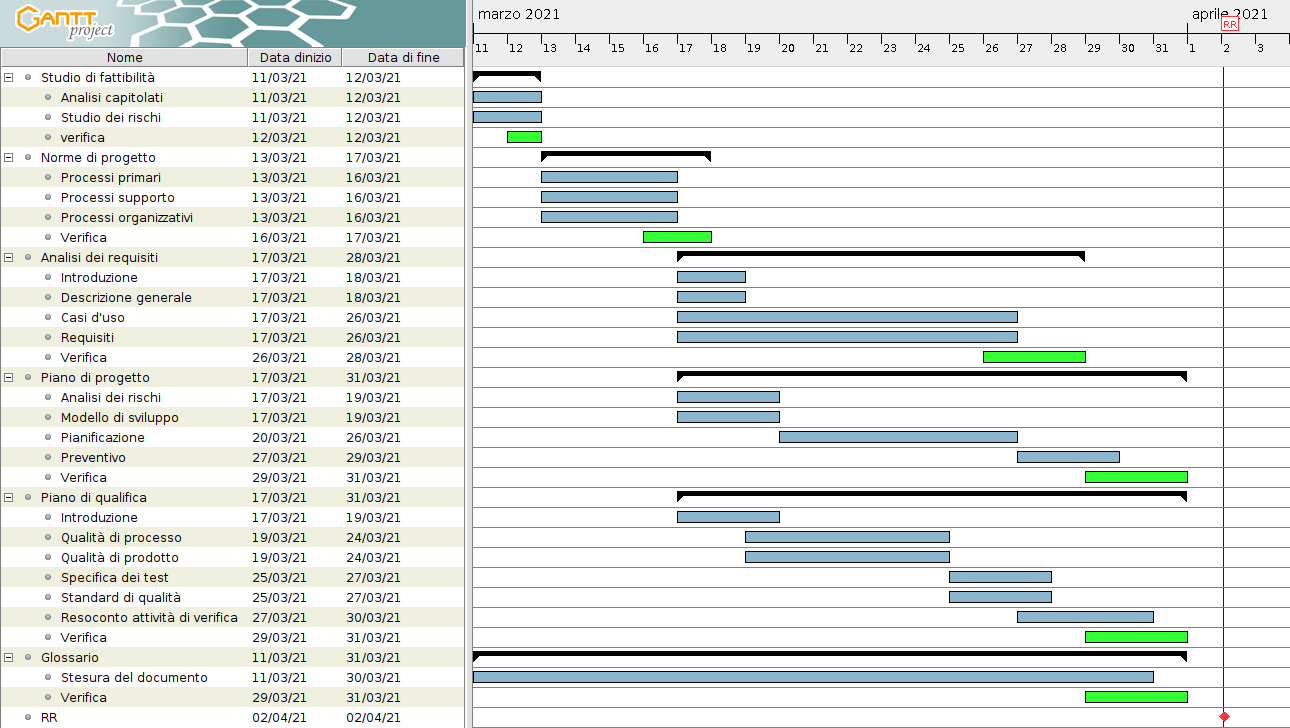
\includegraphics[scale=0.21]{../../../Images/Diagrammi/Gantt/diagramma_gantt_analisi_0.2.png}
    \centering
\end{figure}

\subsection{Consolidamento dei requisiti}
\textit{Periodo: dal 2021-04-02 al 2021-04-09}\\
Questa fase comincia con la fine di quella di Analisi e termina il giorno della presentazione della \textit{Revisione dei Requisiti}. Le attività di questa fase sono:
\begin{itemize}
    \item \textbf{Consolidamento:} con lo scopo di consolidare e migliorare i requisiti ottenuti nella fase precedente;
    \item \textbf{Preparazione alla presentazione:} per preparare il materiale necessario alla presentazione del 2021-04-09;
    \item \textbf{Incremento e Verifica:} nella quale vengono migliorati i documenti prodotti nella fase precedente se necessario;
    \item \textbf{Approfondimento personale:} ogni componente del gruppo dovrà dedicare delle ore di studio autonomo e approfondimento riguardo alle tecnologie necessarie per sviluppare il prodotto.
\end{itemize}
\begin{figure}[!ht]
    \caption{Diagramma di Gantt della fase di consolidamento dei requisiti}
    \vspace{5px}
    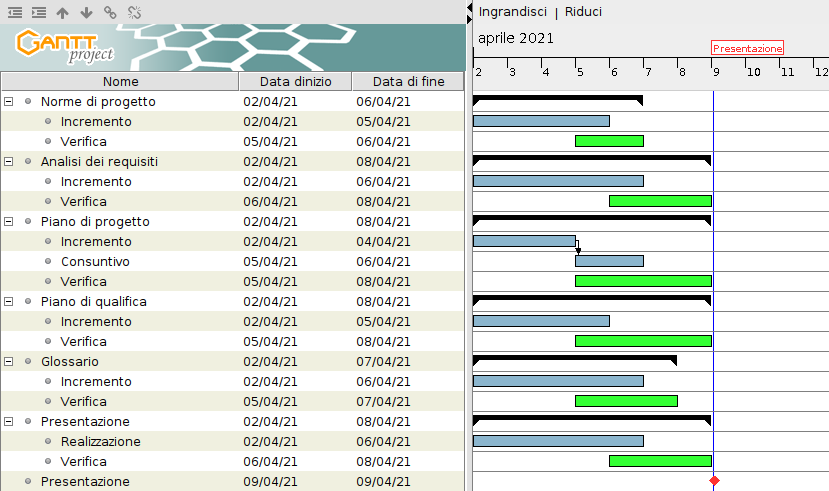
\includegraphics[scale=0.4]{../../../Images/Diagrammi/Gantt/consolidamento.png}
    \centering
\end{figure}
\pagebreak
\subsection{Progettazione architetturale}
\textit{Periodo: dal 2021-04-09 al 2021-05-03}\\
Questa fase comincia il giorno successivo alla presentazione e la sua fine coincide con la data di consegna della \textit{Revisione di Progettazione}. In questo lasso di tempo verrà individuata una soluzione architetturale che soddisfi i requisiti richiesti.\\
Le attività di questa fase sono:
\begin {itemize}
\item \textbf{Incremento e verifica:} in cui i documenti precedentemente redatti vengono aggiornati e migliorati;
\item \textbf{Technology Baseline\textsubscript{\textbf{G}}:} viene fatta un'analisi ad alto livello per comprendere appieno le tecnologie coinvolte, scegliendo l'architettura del codice e i design pattern\textsubscript{\textbf{G}} che saranno adoperati per lo sviluppo. Viene codificato il Proof of Concept\textsubscript{\textbf{G}} che sarà presentato o condiviso tramite repository con committente e proponente per verificare il corretto sviluppo del software.
\end {itemize}
\begin{figure}[!ht]
    \caption{Diagramma di Gantt dell'attività di progettazione architetturale}
    \vspace{5px}
    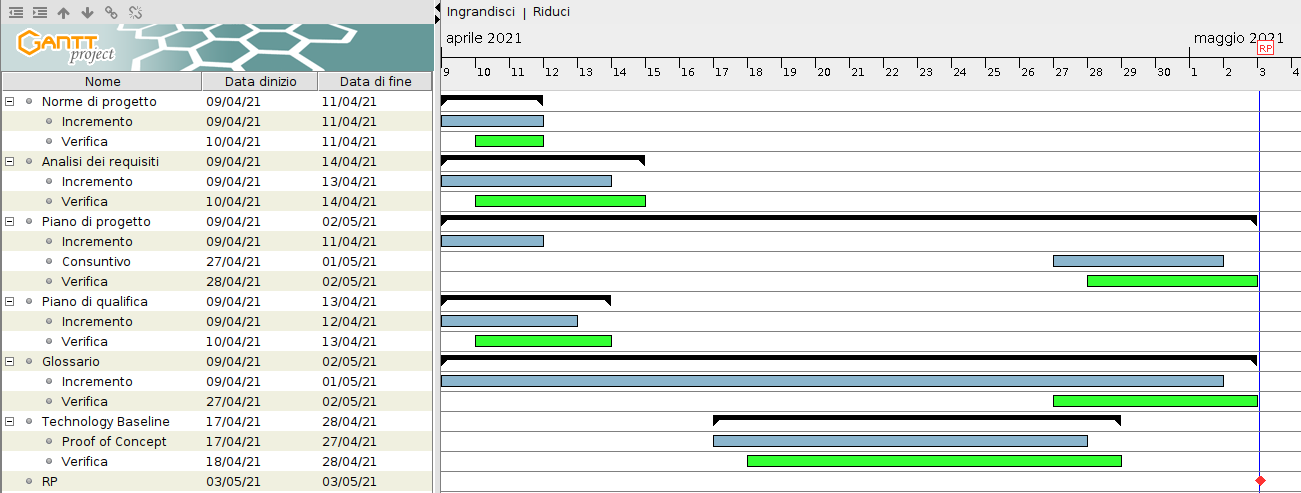
\includegraphics[scale=0.3]{../../../Images/Diagrammi/Gantt/progettArchitetturale_v2.png}
    \centering
\end{figure}

\subsection{Progettazione di dettaglio e codifica}
\textit{Periodo: dal 2021-05-10 al 2021-06-04}\\
L'inizio di questa fase è il giorno della scadenza della \textit{Revisione di Progettazione} e la data di fine coincide con la data di consegna dei documenti in vista della \textit{Revisione di Qualifica}.\\
Le attività di questa fase sono suddivisi in sette incrementi di sviluppo, per ognuno dei quali sono riportate le seguenti voci:
\begin{itemize}
    \item obbiettivi
          \begin{itemize}
              \item software;
              \item documentali;
          \end{itemize}
    \item periodo;
    \item ruoli attivi;
    \item attività previste;
    \item diagramma di Gantt.
\end{itemize}

%Incremento 1 RQ ---------------------------------------------------------
\subsubsection{Incremento 6}
\subsubsubsection{Obbiettivi}
Gli obbiettivi che il gruppo di pone di soddisfare in questo periodo sono i seguenti:
\begin{itemize}
    \item Preparazione alle attività di progettazione e codifica di dettaglio;
    \item Incremento della documentazione per verifica e miglioramento continuo.
\end{itemize}
\subsubsubsection{Periodo}
Il gruppo ritiene che per il raggiungimento degli obbiettivi serviranno quattro giorni di lavoro;\\
Il periodo interessato sarà dal 2021/05/10 al 2021/05/13
\subsubsubsection{Ruoli attivi}
Il gruppo ritiene che durante questo incremento saranno attivi i seguenti ruoli:
\begin{itemize}
    \item \textit{Responsabile di progetto};
    \item \textit{Amministratore di progetto};
    \item \textit{Progettista};
    \item \textit{Verificatore}.
\end{itemize}
\subsubsubsection{Attività previste}
Per soddisfare gli obbiettivi preposti il gruppo ritiene di dover svolgere le seguenti attività:
\begin{itemize}
    \item\textbf{integrazione strumenti:} integrazione degli strumenti necessari allo
          sviluppo del prodotto secondo gli standard qualitativi scelti;
    \item\textbf{analisi delle tecnologie:} studio delle tecnologie necessarie per lo sviluppo software;
    \item \textbf{verifica:} rilevazione delle metriche di qualità di prodotto e di processo;
    \item \textbf{ampliamento della documentazione:}
          \begin{itemize}
              \item estensione delle normative di progettazione e codifica;
              \item aggiornamento delle metriche e degli obbiettivi di qualità per quanto concerne il prodotto software;
              \item registrazione degli esiti di verifica;
              \item registrazione dell'andamento degli obbiettivi di qualità;
              \item aggiornamento dell'analisi dei rischi e della sua attualizzazione;
              \item aggiornamento del \textit{Glossario v3.0.0};
              \item calcolo del consuntivo di periodo;
              \item calcolo del preventivo a finire rispetto alla fase;
              \item calcolo del preventivo a finire rispetto al completamento del progetto.
          \end{itemize}
\end{itemize}

\subsubsubsection{Diagramma di Gantt}
\begin{figure}[!ht]
    \caption{Diagramma di Gantt dell'incremento 6}
    \vspace{5px}
    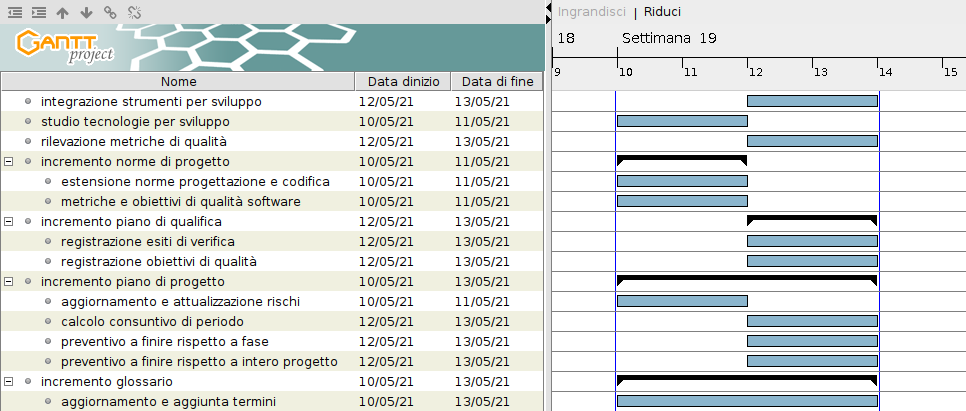
\includegraphics[scale=0.3]{../../../Images/Diagrammi/Gantt/incremento6.png}
    \centering
\end{figure}

%Incremento 2 RQ ---------------------------------------------------------
\subsubsection{Incremento 7}
\subsubsubsection{Obbiettivi}
Gli obbiettivi che il gruppo di pone di soddisfare in questo periodo sono i seguenti:
\begin{itemize}
    \item Miglioramento della struttura delle funzioni Lambda, con l'aggiunta dei filtri di ricerca;
    \item Miglioramento delle chiamate \textit{API GATEWAY} nel frontend per ottenere le informazioni delle funzioni lambda;
    \item Inizio della stesura della documentazione legata al prodotto software;
    \item Incremento della documentazione per verifica e miglioramento continuo.
\end{itemize}
\subsubsubsection{Periodo}
Il gruppo ritiene che per il raggiungimento degli obbiettivi serviranno quattro giorni di lavoro;\\
Il periodo interessato sarà dal 2021/05/14 al 2021/05/17
\subsubsubsection{Ruoli attivi}
Il gruppo ritiene che durante questo incremento saranno attivi i seguenti ruoli:
\begin{itemize}
    \item \textit{Responsabile di progetto};
    \item \textit{Amministratore di progetto};
    \item \textit{Progettista};
    \item \textit{Programmatore};
    \item \textit{Verificatore}.
\end{itemize}
\subsubsubsection{Attività previste}
Per soddisfare gli obbiettivi preposti il gruppo ritiene di dover svolgere le seguenti attività:
\begin{itemize}
    \item \textbf{codifica:}
          \begin{itemize}
              \item implementazione dei casi d'uso UC15- Scelta della categoria e UC35 - Applicazione dei filtri;\\ requisiti:
                    \begin{itemize}
                        \item R10F;                                                                   \item R10.1F
                        \item R10.2F;
                        \item R10.5F;
                        \item R10.6F.
                    \end{itemize}
          \end{itemize}
    \item \textbf{pianificazione:} revisione della modalità di pianificazione gestendola attraverso gli incrementi;
    \item \textbf{progettazione di dettaglio:} inizio della stesura dell'\textit{Allegato Tecnico}:
          \begin{itemize}
              \item esposizione delle tecnologie;
              \item individuazione dei design pattern e della struttura del codice.
          \end{itemize}
    \item \textbf{verifica:} rilevazione delle metriche di qualità di prodotto e di processo;
    \item \textbf{ampliamento della documentazione:}
          \begin{itemize}
              \item inizio stesura \textit{Maintainer Manual v1.0.0} per le funzionalità complete;
              \item inizio stesura \textit{User Manual v1.0.0} per le funzionalità complete;
              \item registrazione degli esiti di verifica;
              \item registrazione dell'andamento degli obbiettivi di qualità;
              \item aggiornamento dell'analisi dei rischi e della sua attualizzazione;
              \item aggiornamento del \textit{Glossario v3.0.0};
              \item calcolo del consuntivo di periodo;
              \item calcolo del preventivo a finire rispetto alla fase;
              \item calcolo del preventivo a finire rispetto al completamento del progetto.
          \end{itemize}
\end{itemize}
\subsubsubsection{Diagramma di Gantt}
\begin{figure}[!ht]
    \caption{Diagramma di Gantt dell'incremento 7}
    \vspace{5px}
    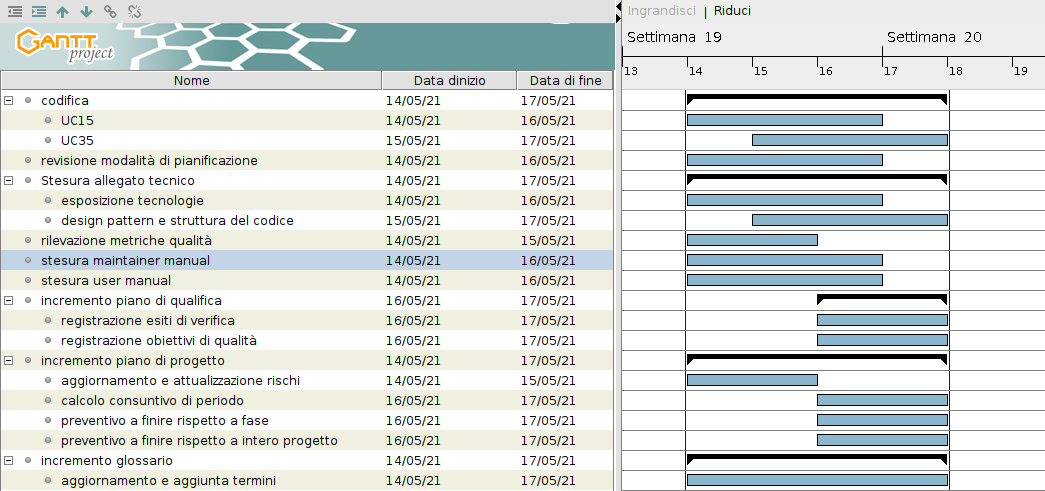
\includegraphics[scale=0.3]{../../../Images/Diagrammi/Gantt/incremento7.png}
    \centering
\end{figure}

%Incremento 3 RQ ---------------------------------------------------------
\subsubsection{Incremento 8}
\subsubsubsection{Obbiettivi}
Gli obbiettivi che il gruppo di pone di soddisfare in questo periodo sono i seguenti:
\begin{itemize}
    \item Ristrutturazione dei servizi lato backend;
    \item Riconfigurazione del linter \textit{eslint};
    \item Correzione della documentazione in base alla RP;
    \item Incremento della documentazione per verifica e miglioramento continuo.
\end{itemize}
\subsubsubsection{Periodo}
Il gruppo ritiene che per il raggiungimento degli obbiettivi serviranno tre giorni di lavoro;\\
Il periodo interessato sarà dal 2021/05/18 al 2021/05/20
\subsubsubsection{Ruoli attivi}
Il gruppo ritiene che durante questo incremento saranno attivi i seguenti ruoli:
\begin{itemize}
    \item \textit{Responsabile di progetto};
    \item \textit{Amministratore di progetto};
    \item \textit{Progettista};
    \item \textit{Programmatore};
    \item \textit{Verificatore}.
\end{itemize}
\subsubsubsection{Attività previste}
Per soddisfare gli obbiettivi preposti il gruppo ritiene di dover svolgere le seguenti attività:
\begin{itemize}
    \item \textbf{codifica:} ristrutturazione del codice per rispettare le indicazioni fornite dai proponenti;\\ requisiti:
          \begin{itemize}
              \item R8Q;
              \item R1v;
              \item R2v;
              \item R4v.
          \end{itemize}
    \item \textbf{configurazione linter:} riconfigurazione del linter \textit{eslint} rispettando le indicazioni fornite dai proponenti. Aggiunta del linter ai sistemi di \textit{continuous integration};
    \item \textbf{progettazione di dettaglio}: incremento della stesura dell'\textit{Allegato Tecnico}:
          \begin{itemize}
              \item aggiunta dei diagrammi delle classi;
              \item aggiunta dei diagrammi di sequenza.
          \end{itemize}
    \item \textbf{verifica:} rilevazione delle metriche di qualità di prodotto e di processo;
    \item \textbf{ampliamento della documentazione:}
          \begin{itemize}
              \item incremento della stesura del \textit{Maintainer Manual v1.0.0} per le funzionalità complete;
              \item incremento della stesura del \textit{User Manual v1.0.0} per le funzionalità complete;
              \item registrazione degli esiti di verifica;
              \item registrazione dell'andamento degli obbiettivi di qualità;
              \item aggiornamento dell'analisi dei rischi e della sua attualizzazione;
              \item aggiornamento del \textit{Glossario v3.0.0};
              \item calcolo del consuntivo di periodo;
              \item calcolo del preventivo a finire rispetto alla fase;
              \item calcolo del preventivo a finire rispetto al completamento del progetto.
          \end{itemize}
\end{itemize}
\subsubsubsection{Diagramma di Gantt}
\begin{figure}[!ht]
    \caption{Diagramma di Gantt dell'incremento 8}
    \vspace{5px}
    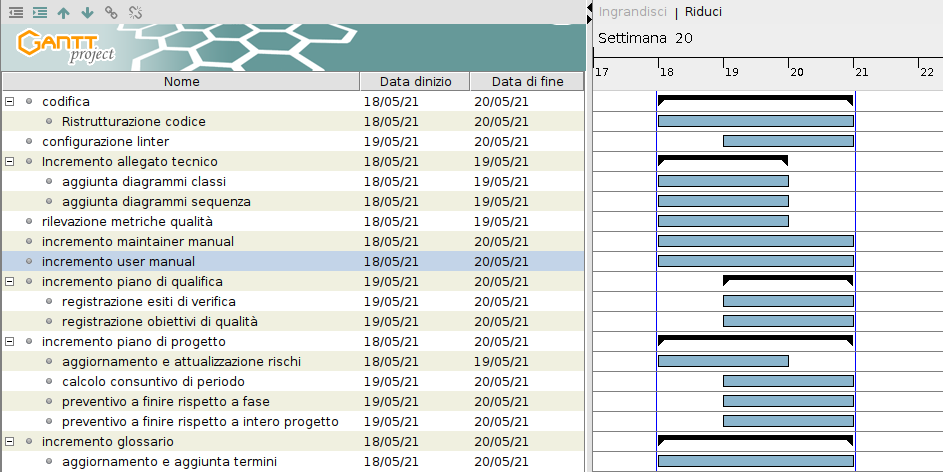
\includegraphics[scale=0.3]{../../../Images/Diagrammi/Gantt/incremento8.png}
    \centering
\end{figure}

%Incremento 4 RQ ---------------------------------------------------------
\subsubsection{Incremento 9}
\subsubsubsection{Obbiettivi}
Gli obbiettivi che il gruppo di pone di soddisfare in questo periodo sono i seguenti:
\begin{itemize}
    \item Distinzione tra cliente e venditore;
    \item Implementazione lato frontend;
    \item Incremento della documentazione per verifica e miglioramento continuo.
\end{itemize}
\subsubsubsection{Periodo}
Il gruppo ritiene che per il raggiungimento degli obbiettivi serviranno due giorni di lavoro;\\
Il periodo interessato sarà dal 2021/05/21 al 2021/05/22
\subsubsubsection{Ruoli attivi}
Il gruppo ritiene che durante questo incremento saranno attivi i seguenti ruoli:
\begin{itemize}
    \item \textit{Responsabile di progetto};
    \item \textit{Amministratore di progetto};
    \item \textit{Progettista};
    \item \textit{Programmatore};
    \item \textit{Verificatore}.
\end{itemize}
\subsubsubsection{Attività previste}
Per soddisfare gli obbiettivi preposti il gruppo ritiene di dover svolgere le seguenti attività:
\begin{itemize}
    \item \textbf{codifica:}
          \begin{itemize}
              \item implementazione del caso d'uso UC17 - Gestione profilo;\\
                    requisiti:
                    \begin{itemize}
                        \item R15F;
                        \item R15.1F;
                        \item R15.2F;
                        \item R15.3F.
                    \end{itemize}
              \item implementazione del caso d'uso UC19 - Visualizzazione profilo;\\
                    requisiti:
                    \begin{itemize}
                        \item R17F.
                    \end{itemize}
              \item implementazione del caso d'uso UC37 - Modifica della password;\\
                    requisiti:
                    \begin{itemize}
                        \item R32F.
                    \end{itemize}
          \end{itemize}
    \item \textbf{progettazione di dettaglio}: incremento della stesura dell'\textit{Allegato Tecnico}:
          \begin{itemize}
              \item aggiunta dei diagrammi di attività.
          \end{itemize}
    \item \textbf{verifica:} rilevazione delle metriche di qualità di prodotto e di processo;
    \item \textbf{ampliamento della documentazione:}
          \begin{itemize}
              \item incremento della stesura del \textit{Maintainer Manual v1.0.0} per le funzionalità complete;
              \item incremento della stesura del \textit{User Manual v1.0.0} per le funzionalità complete;
              \item registrazione degli esiti di verifica;
              \item registrazione dell'andamento degli obbiettivi di qualità;
              \item aggiornamento dell'analisi dei rischi e della sua attualizzazione;
              \item aggiornamento del \textit{Glossario v3.0.0};
              \item calcolo del consuntivo di periodo;
              \item calcolo del preventivo a finire rispetto alla fase;
              \item calcolo del preventivo a finire rispetto al completamento del progetto.
          \end{itemize}
\end{itemize}
\pagebreak
\subsubsubsection{Diagramma di Gantt}
\begin{figure}[!ht]
    \caption{Diagramma di Gantt dell'incremento 9}
    \vspace{5px}
    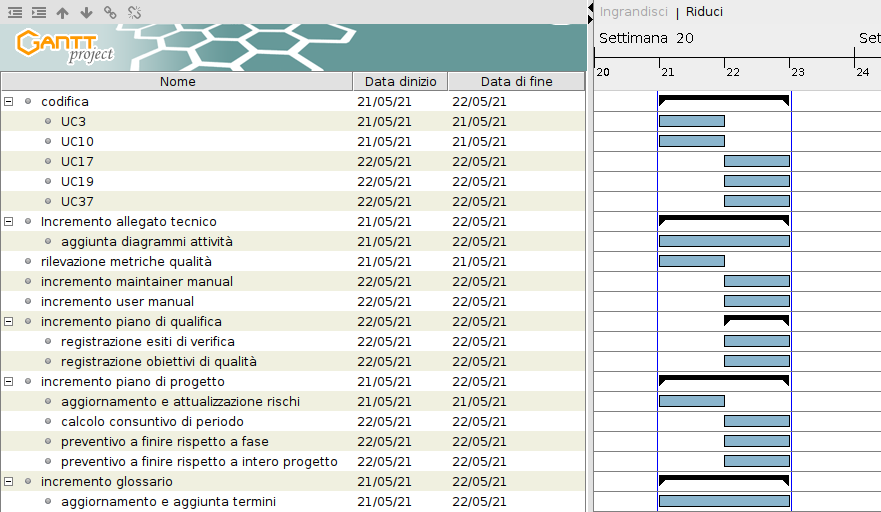
\includegraphics[scale=0.3]{../../../Images/Diagrammi/Gantt/incremento9.png}
    \centering
\end{figure}

%Incremento 5 RQ ---------------------------------------------------------
\subsubsection{Incremento 10}
\subsubsubsection{Obbiettivi}
Gli obbiettivi che il gruppo di pone di soddisfare in questo periodo sono i seguenti:
\begin{itemize}
    \item Completamento Checkout;
    \item Completamento carrello;
    \item Completamento pagina PDP;
    \item Incremento della documentazione per verifica e miglioramento continuo.
\end{itemize}
\subsubsubsection{Periodo}
Il gruppo ritiene che per il raggiungimento degli obbiettivi serviranno tre giorni di lavoro;\\
Il periodo interessato sarà dal 2021/05/23 al 2021/05/25
\subsubsubsection{Ruoli attivi}
Il gruppo ritiene che durante questo incremento saranno attivi i seguenti ruoli:
\begin{itemize}
    \item \textit{Responsabile di progetto};
    \item \textit{Amministratore di progetto};
    \item \textit{Progettista};
    \item \textit{Programmatore};
    \item \textit{Verificatore}.
\end{itemize}
\subsubsubsection{Attività previste}
Per soddisfare gli obbiettivi preposti il gruppo ritiene di dover svolgere le seguenti attività:
\begin{itemize}
    \item \textbf{codifica:}
          \begin{itemize}
              \item implementazione del caso d'uso UC4 - Visualizzazione dettagli di un prodotto;\\
                    requisiti:
                    \begin{itemize}
                        \item R5F;
                        \item R5.8F.
                    \end{itemize}
              \item implementazione del caso d'uso UC5 - Aggiunta di un prodotto al carrello;\\
                    requisiti:
                    \begin{itemize}
                        \item R6F.
                    \end{itemize}
              \item implementazione del caso d'uso UC11 - Visualizzazione dei prodotti inseriti nel carrello;\\
                    requisiti:
                    \begin{itemize}
                        \item R13.5F.
                    \end{itemize}
              \item implementazione del caso d'uso UC12 - Rimozione di un prodotto dal carrello;\\
                    requisiti:
                    \begin{itemize}
                        \item R13.2F.
                    \end{itemize}
              \item implementazione del caso d'uso UC13 - Modifica della quantità di un prodotto nel carrello;\\
                    requisiti:
                    \begin{itemize}
                        \item R13.3F.
                    \end{itemize}
              \item implementazione del caso d'uso UC14 - Visualizzazione errore quantità superata di un prodotto nel carrello;\\
                    requisiti:
                    \begin{itemize}
                        \item R13.3F.
                    \end{itemize}
              \item implementazione del caso d'uso UC21 - Checkout;\\
                    requisiti:
                    \begin{itemize}
                        \item R19F;
                        \item R19.1F;
                        \item R19.2F.
                    \end{itemize}
              \item implementazione del caso d'uso UC22 -  Annullamento checkout;\\
                    requisiti:
                    \begin{itemize}
                        \item R20F.
                    \end{itemize}
              \item implementazione del caso d'uso UC23 -  Riepilogo ordine;\\
                    requisiti:
                    \begin{itemize}
                        \item R21F.
                    \end{itemize}
              \item implementazione del caso d'uso UC24 - Visualizzazione degli ordini effettuati;\\
                    requisiti:
                    \begin{itemize}
                        \item R22F.
                    \end{itemize}
          \end{itemize}
    \item \textbf{verifica:} rilevazione delle metriche di qualità di prodotto e di processo;
    \item \textbf{ampliamento della documentazione:}
          \begin{itemize}
              \item incremento della stesura del \textit{Maintainer Manual v1.0.0} per le funzionalità complete;
              \item incremento della stesura del \textit{User Manual v1.0.0} per le funzionalità complete;
              \item registrazione degli esiti di verifica;
              \item registrazione dell'andamento degli obbiettivi di qualità;
              \item aggiornamento dell'analisi dei rischi e della sua attualizzazione;
              \item aggiornamento del \textit{Glossario v3.0.0};
              \item calcolo del consuntivo di periodo;
              \item calcolo del preventivo a finire rispetto alla fase;
              \item calcolo del preventivo a finire rispetto al completamento del progetto.
          \end{itemize}
\end{itemize}
\subsubsubsection{Diagramma di Gantt}
\begin{figure}[!ht]
    \caption{Diagramma di Gantt dell'incremento 10}
    \vspace{5px}
    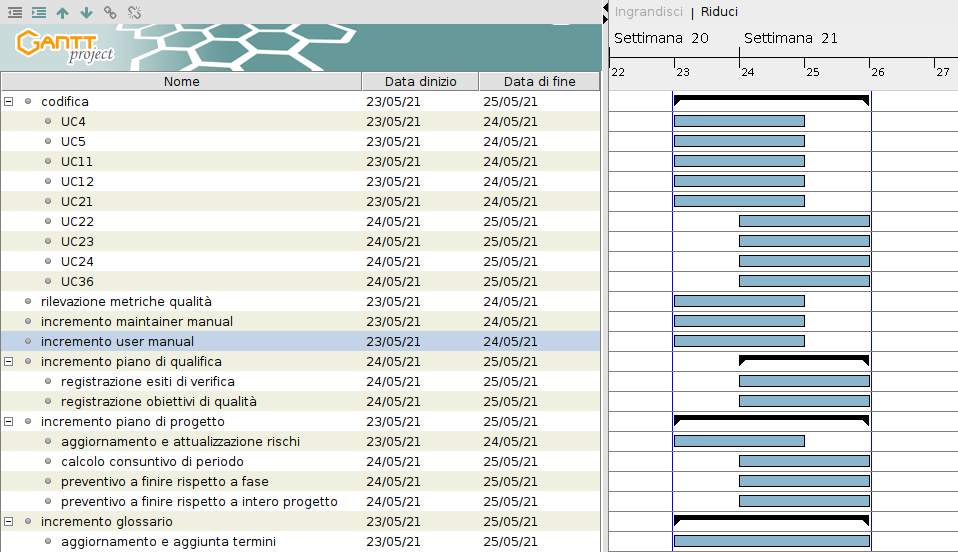
\includegraphics[scale=0.3]{../../../Images/Diagrammi/Gantt/incremento10.png}
    \centering
\end{figure}

%Incremento 6 RQ ---------------------------------------------------------
\subsubsection{Incremento 11}
\subsubsubsection{Obbiettivi}
Gli obbiettivi che il gruppo di pone di soddisfare in questo periodo sono i seguenti:
\begin{itemize}
    \item Completamento Homepage;
    \item Completamento PLP;
    \item Implementazione ricerca di un prodotto;
    \item Incremento della documentazione per verifica e miglioramento continuo.
\end{itemize}
\subsubsubsection{Periodo}
Il gruppo ritiene che per il raggiungimento degli obbiettivi serviranno due giorni di lavoro;\\
Il periodo interessato sarà dal 2021/05/26 al 2021/05/27
\subsubsubsection{Ruoli attivi}
Il gruppo ritiene che durante questo incremento saranno attivi i seguenti ruoli:
\begin{itemize}
    \item \textit{Responsabile di progetto};
    \item \textit{Amministratore di progetto};
    \item \textit{Programmatore};
    \item \textit{Verificatore}.
\end{itemize}
\subsubsubsection{Attività previste}
Per soddisfare gli obbiettivi preposti il gruppo ritiene di dover svolgere le seguenti attività:
\begin{itemize}
    \item \textbf{codifica:}
          \begin{itemize}
              \item completamento implementazione homepage;\\ requisiti:
                    \begin{itemize}
                        \item R1.1F;
                        \item R10.1F;
                        \item R1.2F.
                    \end{itemize}
              \item implementazione dei casi d'uso UC6 - Ricerca dei prodotti;\\ requisiti:
                    \begin{itemize}
                        \item R7F.
                    \end{itemize}
              \item implementazione dei casi d'uso UC7 - Visualizzazione della lista dei prodotti;\\ requisiti:
                    \begin{itemize}
                        \item R8F.
                    \end{itemize}
          \end{itemize}
    \item \textbf{verifica:} rilevazione delle metriche di qualità di prodotto e di processo;
    \item \textbf{ampliamento della documentazione:}
          \begin{itemize}
              \item registrazione degli esiti di verifica;
              \item registrazione dell'andamento degli obbiettivi di qualità;
              \item aggiornamento dell'analisi dei rischi e della sua attualizzazione;
              \item aggiornamento del \textit{Glossario v3.0.0};
              \item calcolo del consuntivo di periodo;
              \item calcolo del preventivo a finire rispetto alla fase;
              \item calcolo del preventivo a finire rispetto al completamento del progetto.
          \end{itemize}
\end{itemize}

\subsubsubsection{Diagramma di Gantt}
\begin{figure}[!ht]
    \caption{Diagramma di Gantt dell'incremento 11}
    \vspace{5px}
    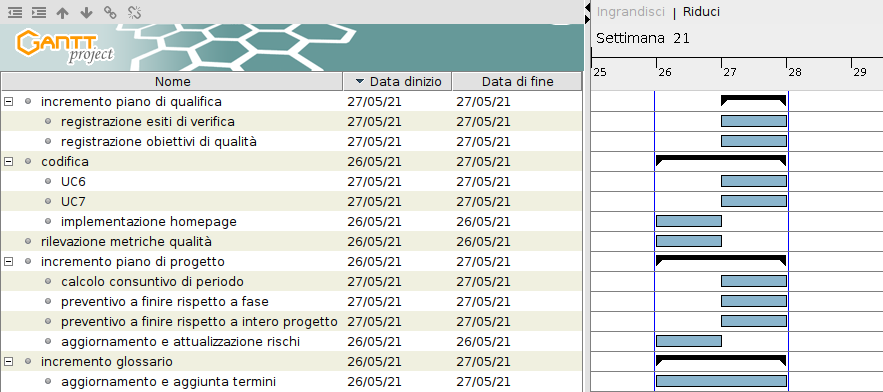
\includegraphics[scale=0.3]{../../../Images/Diagrammi/Gantt/incremento11.png}
    \centering
\end{figure}

%Incremento 7 RQ ---------------------------------------------------------
\subsubsection{Incremento 12}
\subsubsubsection{Obbiettivi}
\begin{itemize}
    \item Completamento pagina venditore;
    \item Aggiunta sezione per la gestione delle categorie;
    \item Aggiunta visualizzazione elenco clienti e ordini ricevuti;
    \item Aggiunta sezione per la gestione di un prodotto;
    \item Incremento della documentazione per verifica e miglioramento continuo.
\end{itemize}
Gli obbiettivi che il gruppo di pone di soddisfare in questo periodo sono i seguenti:
\subsubsubsection{Periodo}
Il gruppo ritiene che per il raggiungimento degli obbiettivi serviranno tre giorni di lavoro;\\
Il periodo interessato sarà dal 2021/05/28 al 2021/05/30
\subsubsubsection{Ruoli attivi}
Il gruppo ritiene che durante questo incremento saranno attivi i seguenti ruoli:
\begin{itemize}
    \item \textit{Responsabile di progetto};
    \item \textit{Amministratore di progetto};
    \item \textit{Programmatore};
    \item \textit{Verificatore}.
\end{itemize}
\subsubsubsection{Attività previste}
Per soddisfare gli obbiettivi preposti il gruppo ritiene di dover svolgere le seguenti attività:
\begin{itemize}
    \item \textbf{codifica:}
          \begin{itemize}
              \item implementazione del caso d'uso UC25 - Visualizzazione della lista dei clienti;\\
                    requisiti:
                    \begin{itemize}
                        \item R23F.
                    \end{itemize}
              \item implementazione del caso d'uso UC26 - Visualizzazione della lista degli ordini;\\
                    requisiti:
                    \begin{itemize}
                        \item R24F.
                    \end{itemize}
              \item implementazione del caso d'uso UC28 -  Aggiunta di un prodotto;\\
                    requisiti:
                    \begin{itemize}
                        \item R26F.
                    \end{itemize}
              \item implementazione del caso d'uso UC29 - Modifica di un prodotto;\\
                    requisiti:
                    \begin{itemize}
                        \item R27F.
                    \end{itemize}
              \item implementazione del caso d'uso UC30 - Rimozione di un prodotto;\\
                    requisiti:
                    \begin{itemize}
                        \item R28F.
                    \end{itemize}
              \item implementazione del caso d'uso UC31 -  Aggiunta di una categoria;\\
                    requisiti:
                    \begin{itemize}
                        \item R29F.
                    \end{itemize}
              \item implementazione del caso d'uso UC32 -  Rimozione di una categoria;\\
                    requisiti:
                    \begin{itemize}
                        \item R30F.
                    \end{itemize}
          \end{itemize}
    \item \textbf{verifica:} rilevazione delle metriche di qualità di prodotto e di processo;
    \item \textbf{ampliamento della documentazione:}
          \begin{itemize}
              \item registrazione degli esiti di verifica;
              \item registrazione dell'andamento degli obbiettivi di qualità;
              \item aggiornamento dell'analisi dei rischi e della sua attualizzazione;
              \item aggiornamento del \textit{Glossario v3.0.0};
              \item calcolo del consuntivo di periodo;
              \item calcolo del preventivo a finire rispetto alla fase;
              \item calcolo del preventivo a finire rispetto al completamento del progetto.
          \end{itemize}
\end{itemize}
\subsubsubsection{Diagramma di Gantt}
\begin{figure}[!ht]
    \caption{Diagramma di Gantt dell'incremento 12}
    \vspace{5px}
    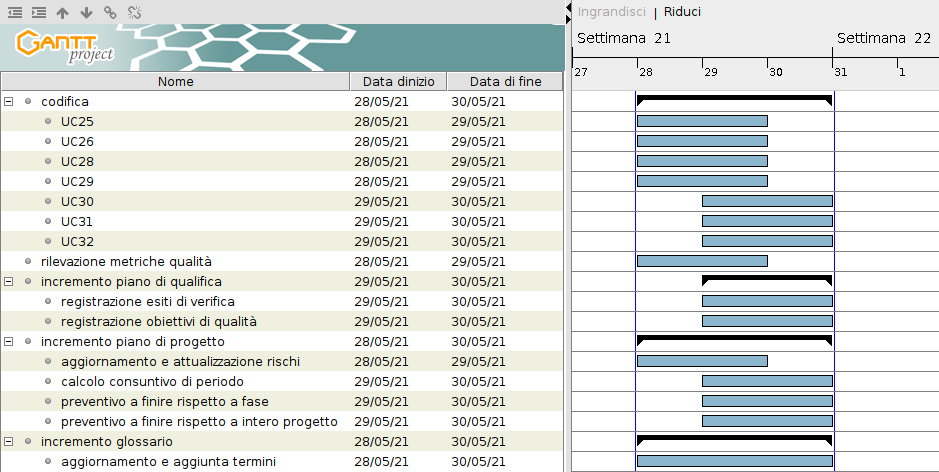
\includegraphics[scale=0.3]{../../../Images/Diagrammi/Gantt/incremento12.png}
    \centering
\end{figure}

%Incremento 8 RQ ---------------------------------------------------------
\subsubsection{Incremento 13}
\subsubsubsection{Obbiettivi}
Gli obbiettivi che il gruppo di pone di soddisfare in questo periodo sono i seguenti:
\begin{itemize}
    \item Preparazione per la \textit{Revisione di Qualifica};
    \item Correzione del codice secondo le indicazioni ricevute durante la \textit{Product Baseline} e con il proponente;
    \item Correzione dell'\textbf{Allegato Tecnico};
    \item Incremento della documentazione per verifica e miglioramento continuo.
\end{itemize}
\subsubsubsection{Periodo}
Il gruppo ritiene che per il raggiungimento degli obbiettivi serviranno quattro giorni di lavoro;\\
Il periodo interessato sarà dal 2021/05/31 al 2021/06/03
\subsubsubsection{Ruoli attivi}
Il gruppo ritiene che durante questo incremento saranno attivi i seguenti ruoli:
\begin{itemize}
    \item \textit{Responsabile di progetto};
    \item \textit{Amministratore di progetto};
    \item \textit{Programmatore};
    \item \textit{Verificatore}.
\end{itemize}
\subsubsubsection{Attività previste}
Per soddisfare gli obbiettivi preposti il gruppo ritiene di dover svolgere le seguenti attività:
\begin{itemize}
    \item\textbf{codifica:}
    \item \begin{itemize}
              \item correzione in base alle indicazioni ricevute durante la \textit{Product Baseline};
              \item correzione in base alle indicazioni ricevute dal proponente.
          \end{itemize}
    \item \textbf{verifica:} rilevazione delle metriche di qualità di prodotto e di processo;
    \item \textbf{ampliamento della documentazione:}
          \begin{itemize}
              \item registrazione degli esiti di verifica;
              \item registrazione dell'andamento degli obbiettivi di qualità;
              \item aggiornamento dell'analisi dei rischi e della sua attualizzazione;
              \item aggiornamento del \textit{Glossario v3.0.0};
              \item calcolo del consuntivo di periodo;
              \item calcolo del preventivo a finire rispetto alla fase;
              \item calcolo del preventivo a finire rispetto al completamento del progetto.
          \end{itemize}
\end{itemize}
\subsubsubsection{Diagramma di Gantt}
\begin{figure}[!ht]
    \caption{Diagramma di Gantt dell'incremento 13}
    \vspace{5px}
    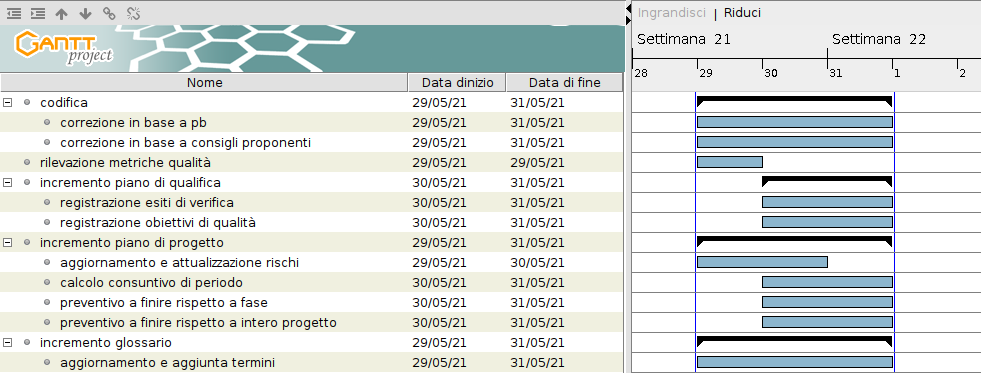
\includegraphics[scale=0.3]{../../../Images/Diagrammi/Gantt/incremento13.png}
    \centering
\end{figure}

% \begin{itemize}
%     \item \textbf{Incremento e verifica:} in cui i documenti precedentemente redatti vengono aggiornati e migliorati;
%     \item \textbf{Product Baseline\textsubscript{\textbf{G}}}: a seguito della \textit{Technology Baseline} l'architettura individuata in essa viene scomposta nelle sue unità, che vengono analizzate in profondità per fornire i dettagli necessari alla loro codifica e verifica;
%     \item \textbf{Codifica:} questa attività consiste nella scrittura e verifica del codice secondo i modi definiti nel \textit{Piano di Qualifica v2.0.0}.
%     \item \textbf{Specifica Tecnica:} Viene redatto un documento contenente tutte le caratteristiche del prodotto e le motivazioni che hanno portato alla loro scelta;
%     \item \textbf{User Manual:} viene redatto un documento contenente le istruzioni d'uso del software da parte dell'utente.
% \end{itemize}
\subsubsection{Diagramma di Gantt della fase}
In base alle attività pianificate negli incrementi e alla loro distribuzione nel tempo, la pianificazione complessiva della fase può essere riassunta nel seguente diagramma.
\begin{figure}[!ht]
    \caption{Diagramma di Gantt dell'attività di progettazione di dettaglio e codifica}
    \vspace{5px}
    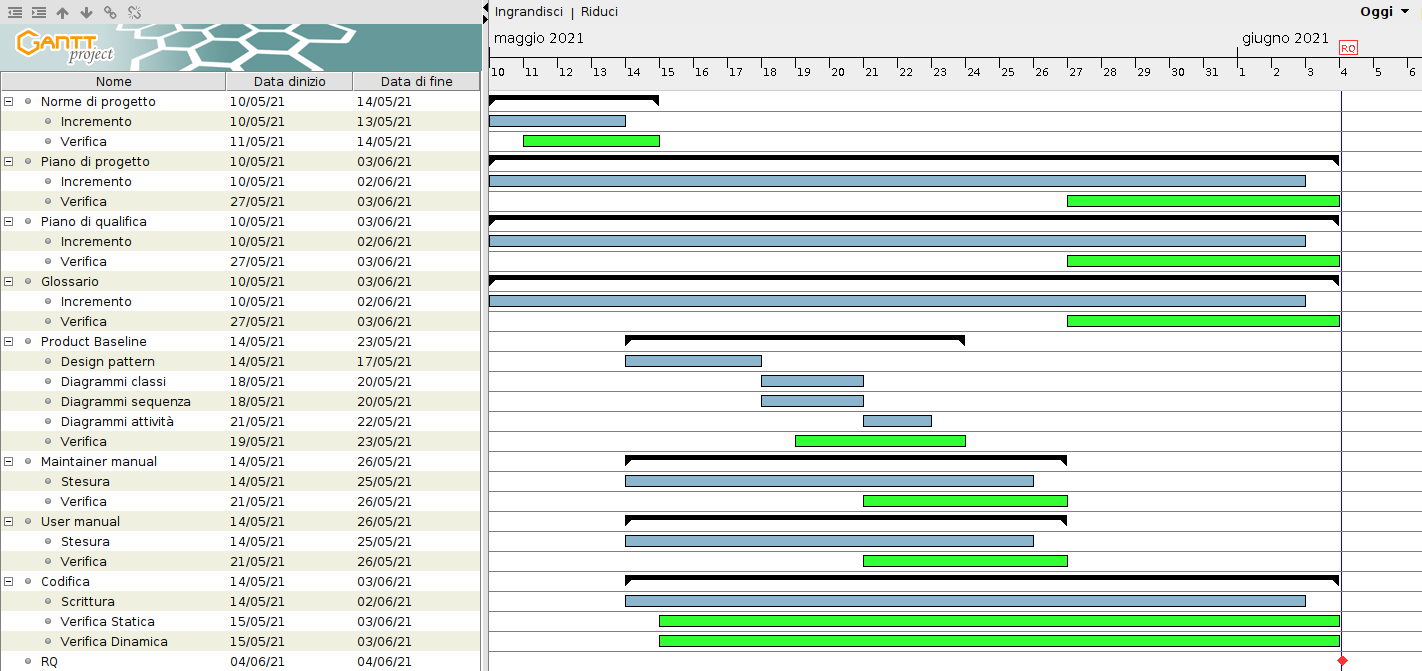
\includegraphics[scale=0.22]{../../../Images/Diagrammi/Gantt/progettazioneCodifica_v3.png}
    \centering
\end{figure}

\subsection{Validazione e collaudo}
\textit{Periodo: dal 2021-07-09 al 2021-08-23}\\
L'inizio di questa fase è il giorno della scadenza della \textit{Revisione di Qualifica} e la data di fine coincide con la data di consegna dei documenti in vista della \textit{Revisione di Accettazione}.\\
Le attività di questa fase sono:
\begin{itemize}
    \item \textbf{Incremento e verifica:} in cui i documenti precedentemente redatti vengono aggiornati e migliorati;
    \item \textbf{Validazione e collaudo:} per la parte di collaudo si eseguiranno ulteriori test sul prodotto, in modo da garantirne correttezza e stabilità. Per ciò che concerne la validazione, verrà valutata la coerenza del prodotto e dei requisiti specificati nel documento \textit{Analisi dei Requisiti} nella sua ultima versione;
\end{itemize}
Le attività di questa fase sono suddivise in quattro incrementi di sviluppo, per ognuno dei quali sono riportate le seguenti voci:
\begin{itemize}
    \item obbiettivi
          \begin{itemize}
              \item software;
              \item documentali;
          \end{itemize}
    \item periodo;
    \item ruoli attivi;
    \item attività previste;
    \item diagramma di Gantt.
\end{itemize}

%Incremento 1 RA ---------------------------------------------------------
\subsubsection{Incremento 14}
\subsubsubsection{Obbiettivi}
Gli obbiettivi che il gruppo di pone di soddisfare in questo periodo sono i seguenti:
\begin{itemize}
    \item Aggiunta ordinamento alla lista dei prodotti;
    \item Aggiunti filtri per categoria e marca;
    \item Aggiunto acquisto diretto del prodotto;;
    \item Incremento della documentazione per verifica e miglioramento continuo.
\end{itemize}
\subsubsubsection{Periodo}
Il gruppo ritiene che per il raggiungimento degli obbiettivi serviranno dieci giorni di lavoro;\\
Il periodo interessato sarà dal 2021/07/09 al 2021/07/18
\subsubsubsection{Ruoli attivi}
Il gruppo ritiene che durante questo incremento saranno attivi i seguenti ruoli:
\begin{itemize}
    \item \textit{Responsabile di progetto};
    \item \textit{Amministratore di progetto};
    \item \textit{Progettista};
    \item \textit{Programmatore};
    \item \textit{Verificatore}.
\end{itemize}
\subsubsubsection{Attività previste}
Per soddisfare gli obbiettivi preposti il gruppo ritiene di dover svolgere le seguenti attività:
\begin{itemize}
    \item implementazione del caso d'uso UC4 - Acquisto diretto del prodotto;\\requisiti:
          \begin{itemize}
              \item R5.9F.
          \end{itemize}
    \item implementazione del caso d'uso UC15 - Scelta della categoria;\\requisiti:
          \begin{itemize}
              \item R10.4F.
          \end{itemize}
    \item implementazione del caso d'uso UC34 - Ordinamento prodotti;\\requisiti:
          \begin{itemize}
              \item R9F;
              \item R9.1F;
              \item R9.2F.
          \end{itemize}
    \item implementazione del caso d'uso UC35 - Applicazione filtri;\\requisiti:
          \begin{itemize}
              \item R10.3F.
          \end{itemize}
    \item \textbf{verifica:} rilevazione delle metriche di qualità di prodotto e di processo;
    \item \textbf{ampliamento della documentazione:}
          \begin{itemize}
              \item incremento della stesura del \textit{Maintainer Manual v2.0.0} per le funzionalità complete;
              \item incremento della stesura del \textit{User Manual v2.0.0} per le funzionalità complete;
              \item aggiornamento delle metriche e degli obbiettivi di qualità per quanto concerne il prodotto software;
              \item registrazione degli esiti di verifica;
              \item registrazione dell'andamento degli obbiettivi di qualità;
              \item aggiornamento dell'analisi dei rischi e della sua attualizzazione;
              \item aggiornamento del \textit{Glossario v4.0.0};
              \item calcolo del consuntivo di periodo;
              \item calcolo del preventivo a finire rispetto alla fase;
              \item calcolo del preventivo a finire rispetto al completamento del progetto.
          \end{itemize}
\end{itemize}
\pagebreak
\subsubsubsection{Diagramma di Gantt}
\begin{figure}[!ht]
    \caption{Diagramma di Gantt dell'incremento 14}
    \vspace{5px}
    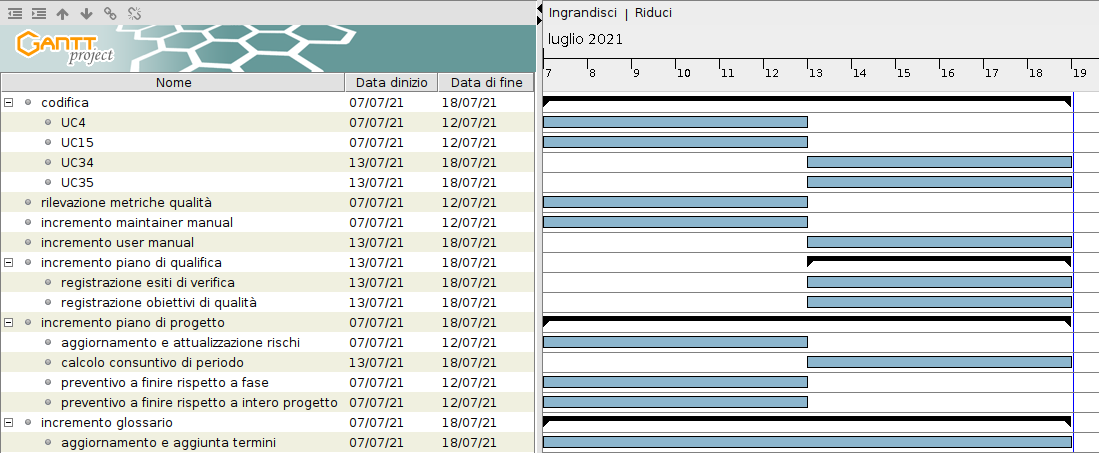
\includegraphics[scale=0.3]{../../../Images/Diagrammi/Gantt/incremento14.png}
    \centering
\end{figure}

%Incremento 2 RA ---------------------------------------------------------
\subsubsection{Incremento 15}
\subsubsubsection{Obbiettivi}
Gli obbiettivi che il gruppo di pone di soddisfare in questo periodo sono i seguenti:
\begin{itemize}
    \item Aggiunta gestione della quantità dei prodotti all'interno del carrello;
    \item Aggiunto registrazione con servizio esterno;
    \item Aggiunto autenticazione con servizio esterno;
    \item Incremento della documentazione per verifica e miglioramento continuo.
\end{itemize}
\subsubsubsection{Periodo}
Il gruppo ritiene che per il raggiungimento degli obbiettivi serviranno dodici giorni di lavoro;\\
Il periodo interessato sarà dal 2021/07/19 al 2021/07/30
\subsubsubsection{Ruoli attivi}
Il gruppo ritiene che durante questo incremento saranno attivi i seguenti ruoli:
\begin{itemize}
    \item \textit{Responsabile di progetto};
    \item \textit{Amministratore di progetto};
    \item \textit{Progettista};
    \item \textit{Programmatore};
    \item \textit{Verificatore}.
\end{itemize}
\subsubsubsection{Attività previste}
Per soddisfare gli obbiettivi preposti il gruppo ritiene di dover svolgere le seguenti attività:
\begin{itemize}
    \item implementazione del caso d'uso UC3 - Autenticazione esterna;\\requisiti:
          \begin{itemize}
              \item R4F.
          \end{itemize}
    \item implementazione del caso d'uso UC10 - Registrazione esterna;\\requisiti:
          \begin{itemize}
              \item R12F.
          \end{itemize}
    \item \textbf{analisi dei requisiti:} correzione in base alle indicazioni dei committenti ricevute in seguito alla RQ
    \item \textbf{piano di progetto:} correzione in base alle indicazioni dei committenti ricevute in seguito alla RQ
    \item \textbf{norme di progetto:} correzione in base alle indicazioni dei committenti ricevute in seguito alla RQ
    \item \textbf{piano di qualifica:} correzione in base alle indicazioni dei committenti ricevute in seguito alla RQ
    \item \textbf{verifica:} rilevazione delle metriche di qualità di prodotto e di processo;
    \item \textbf{ampliamento della documentazione:}
          \begin{itemize}
              \item incremento della stesura del \textit{Maintainer Manual v2.0.0} per le funzionalità complete;
              \item incremento della stesura del \textit{User Manual v2.0.0} per le funzionalità complete;
              \item aggiornamento delle metriche e degli obbiettivi di qualità per quanto concerne il prodotto software;
              \item registrazione degli esiti di verifica;
              \item registrazione dell'andamento degli obbiettivi di qualità;
              \item aggiornamento dell'analisi dei rischi e della sua attualizzazione;
              \item aggiornamento del \textit{Glossario v4.0.0};
              \item calcolo del consuntivo di periodo;
              \item calcolo del preventivo a finire rispetto alla fase;
              \item calcolo del preventivo a finire rispetto al completamento del progetto.
          \end{itemize}
\end{itemize}
\subsubsubsection{Diagramma di Gantt}
\begin{figure}[!ht]
    \caption{Diagramma di Gantt dell'incremento 15}
    \vspace{5px}
    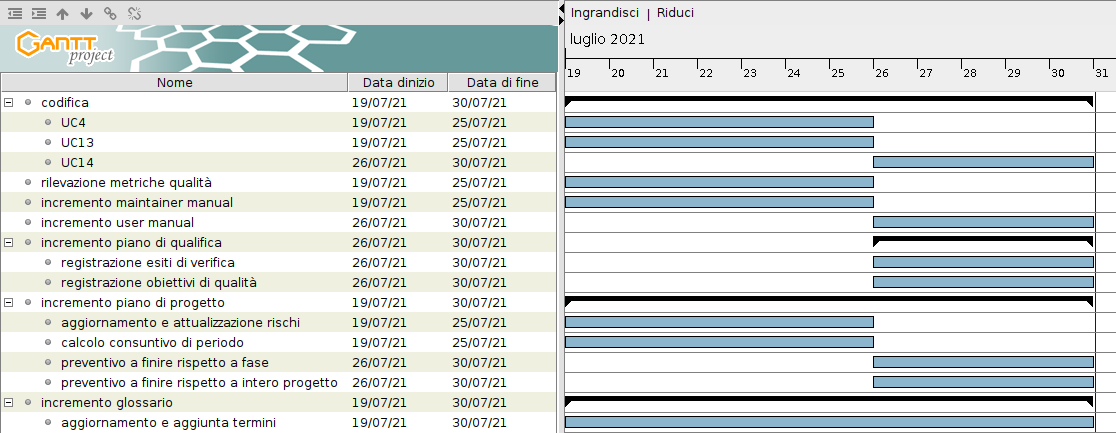
\includegraphics[scale=0.3]{../../../Images/Diagrammi/Gantt/incremento15.png}
    \centering
\end{figure}

%Incremento 3 RA ---------------------------------------------------------
\subsubsection{Incremento 16}
\subsubsubsection{Obbiettivi}
Gli obbiettivi che il gruppo di pone di soddisfare in questo periodo sono i seguenti:
\begin{itemize}
    \item Aggiunto la possibilità d'invio di messaggi tra venditore e cliente;
    \item Incremento della documentazione per verifica e miglioramento continuo.
\end{itemize}
\subsubsubsection{Periodo}
Il gruppo ritiene che per il raggiungimento degli obbiettivi serviranno diciassette giorni di lavoro;\\
Il periodo interessato sarà dal 2021/07/31 al 2021/08/16
\subsubsubsection{Ruoli attivi}
Il gruppo ritiene che durante questo incremento saranno attivi i seguenti ruoli:
\begin{itemize}
    \item \textit{Responsabile di progetto};
    \item \textit{Amministratore di progetto};
    \item \textit{Progettista};
    \item \textit{Programmatore};
    \item \textit{Verificatore}.
\end{itemize}
\subsubsubsection{Attività previste}
Per soddisfare gli obbiettivi preposti il gruppo ritiene di dover svolgere le seguenti attività:
\begin{itemize}
    \item implementazione del caso d'uso UC20 - Contatta il venditore;\\requisiti:
          \begin{itemize}
              \item R18F.
          \end{itemize}
    \item implementazione del caso d'uso UC27 - Contatta un cliente;\\requisiti:
          \begin{itemize}
              \item R25F.
          \end{itemize}
    \item \textbf{verifica:} rilevazione delle metriche di qualità di prodotto e di processo;
    \item \textbf{ampliamento della documentazione:}
          \begin{itemize}
              \item incremento della stesura del \textit{Maintainer Manual v2.0.0} per le funzionalità complete;
              \item incremento della stesura del \textit{User Manual v2.0.0} per le funzionalità complete;
              \item aggiornamento delle metriche e degli obbiettivi di qualità per quanto concerne il prodotto software;
              \item registrazione degli esiti di verifica;
              \item registrazione dell'andamento degli obbiettivi di qualità;
              \item aggiornamento dell'analisi dei rischi e della sua attualizzazione;
              \item aggiornamento del \textit{Glossario v4.0.0};
              \item calcolo del consuntivo di periodo;
              \item calcolo del preventivo a finire rispetto alla fase;
              \item calcolo del preventivo a finire rispetto al completamento del progetto.
          \end{itemize}
\end{itemize}
\pagebreak
\subsubsubsection{Diagramma di Gantt}
\begin{figure}[!ht]
    \caption{Diagramma di Gantt dell'incremento 16}
    \vspace{5px}
    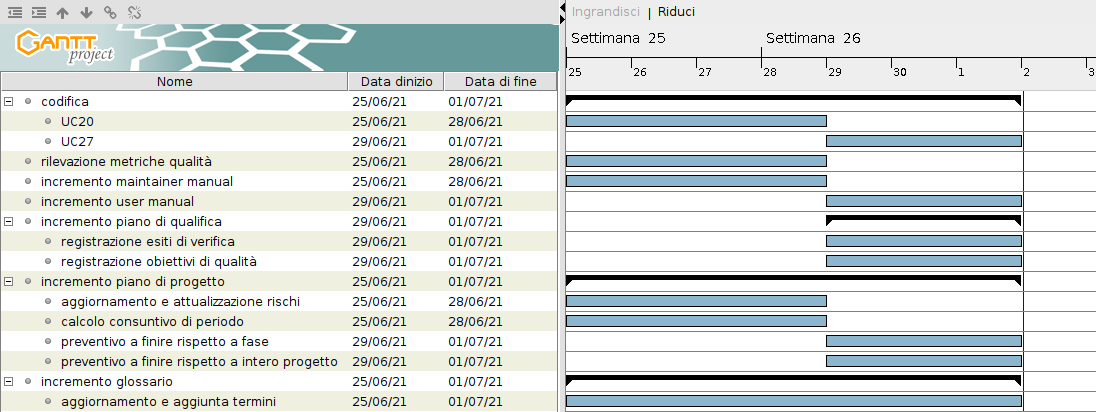
\includegraphics[scale=0.3]{../../../Images/Diagrammi/Gantt/incremento16.png}
    \centering
\end{figure}

%Incremento 4 RA ---------------------------------------------------------
\subsubsection{Incremento 17}
\subsubsubsection{Obbiettivi}
Gli obbiettivi che il gruppo di pone di soddisfare in questo periodo sono i seguenti:
\begin{itemize}
    \item Preparazione all'esposizione per la \textit{Revisione di accettazione};
    \item Preparazione per il collaudo con il proponente;
    \item Incremento della documentazione per verifica e miglioramento continuo.
\end{itemize}
\subsubsubsection{Periodo}
Il gruppo ritiene che per il raggiungimento degli obbiettivi serviranno sei giorni di lavoro;\\
Il periodo interessato sarà dal 2021/08/17 al 2021/08/22
\subsubsubsection{Ruoli attivi}
Il gruppo ritiene che durante questo incremento saranno attivi i seguenti ruoli:
\begin{itemize}
    \item \textit{Responsabile di progetto};
    \item \textit{Amministratore di progetto};
    \item \textit{Progettista};
    \item \textit{Programmatore};
    \item \textit{Verificatore}.
\end{itemize}
\subsubsubsection{Attività previste}
Per soddisfare gli obbiettivi preposti il gruppo ritiene di dover svolgere le seguenti attività:
\begin{itemize}
    \item \textbf{presentazione:} preparazione della presentazione per la \textit{Revisione di Accettazione}, e per il collaudo con il proponente;
    \item \textbf{verifica:} rilevazione delle metriche di qualità di prodotto e di processo;
    \item \textbf{ampliamento della documentazione:}
          \begin{itemize}
              \item estensione delle normative di progettazione e codifica;
              \item aggiornamento delle metriche e degli obbiettivi di qualità per quanto concerne il prodotto software;
              \item registrazione degli esiti di verifica;
              \item registrazione dell'andamento degli obbiettivi di qualità;
              \item aggiornamento dell'analisi dei rischi e della sua attualizzazione;
              \item aggiornamento del \textit{Glossario v4.0.0};
              \item calcolo del consuntivo di periodo;
              \item calcolo del preventivo a finire rispetto alla fase;
              \item calcolo del preventivo a finire rispetto al completamento del progetto.
          \end{itemize}
\end{itemize}

\subsubsubsection{Diagramma di Gantt}
\begin{figure}[!ht]
    \caption{Diagramma di Gantt dell'incremento 17}
    \vspace{5px}
    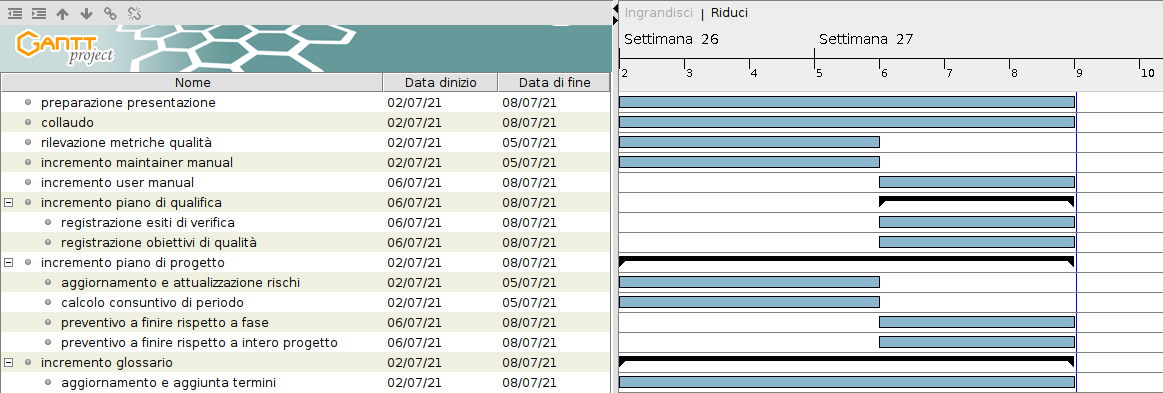
\includegraphics[scale=0.3]{../../../Images/Diagrammi/Gantt/incremento17.png}
    \centering
\end{figure}

\pagebreak
\subsubsection{Diagramma di Gantt della fase}
In base alle attività pianificate negli incrementi e alla loro distribuzione nel tempo, la pianificazione complessiva della fase può essere riassunta nel seguente diagramma.
\begin{figure}[!ht]
    \caption{Diagramma di Gantt dell'attività di Validazione e Collaudo}
    \vspace{5px}
    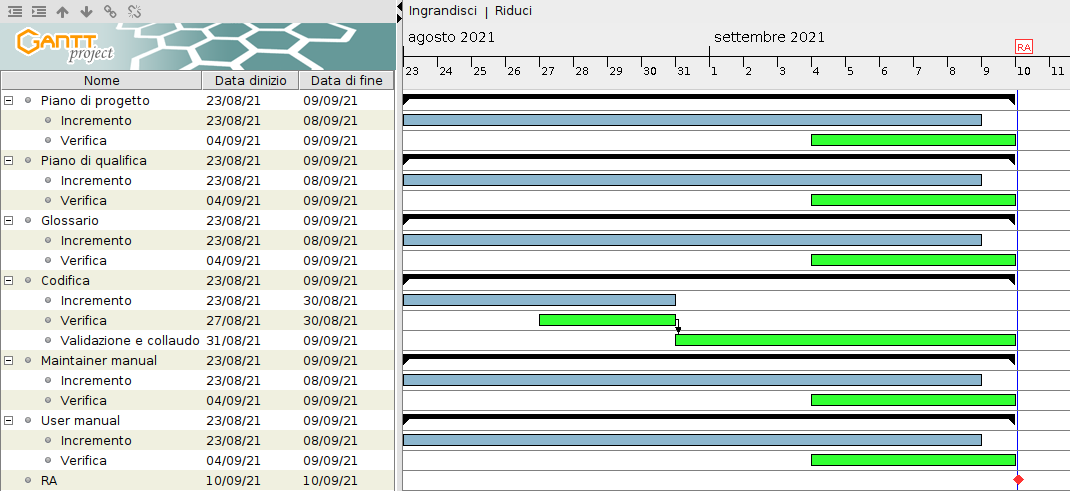
\includegraphics[scale=0.25]{../../../Images/Diagrammi/Gantt/validazione_v3.png}
    \centering
\end{figure}
\section{Preventivo}
Per descrivere come il gruppo \emph{TechSWEave} utilizzerà le risorse a sua disposizione, abbiamo stilato delle tabelle orarie con la suddivisione dei ruoli, utilizzando le seguenti sigle:
\begin{itemize}
    \item \textbf{Re: }\emph{Responsabile};
    \item \textbf{Am: }\emph{Amministratore}
    \item \textbf{An: }\emph{Analista};
    \item \textbf{Pt: }\emph{Progettista};
    \item \textbf{Pr: }\emph{Programmatore};
    \item \textbf{Ve: }\emph{Verificatore};
\end{itemize}

\subsection{Fase di Analisi}
\subsubsection{Prospetto orario}
In questa periodo la distribuzione oraria dei ruoli sarà la seguente:
\begin{center}
    \begin{table}[ht!]
        \centering
        \caption{Distribuzione delle ore della fase di Analisi}
        \vspace{5px}
        \rowcolors{2}{logo!10}{logo!40}
        \renewcommand{\arraystretch}{1.8}
        \begin{tabular}{p{100px} p{20px} p{20px} p{20px} p{20px} p{20px} p{20px} p{50px} }
            \rowcolor{logo!70} \textbf{Nominativo} & \textbf{Re} & \textbf{Am} & \textbf{An} & \textbf{Pt} & \textbf{Pr} & \textbf{Ve} & \textbf{Ore totali} \\
            Marco Barbaresco                       & -           & 10          & 10          & -           & -           & 15          & 35                  \\
            Samuele De Simone                      & 8           & -           & 17          & -           & -           & 10          & 35                  \\
            Nicolò Giaccone                        & -           & 7           & 21          & -           & -           & 7           & 35                  \\
            Amedeo Meggiolaro                      & -           & -           & 18          & -           & -           & 17          & 35                  \\
            Tito Scutari                           & -           & 8           & 12          & -           & -           & 15          & 35                  \\
            Simone Urbani                          & 6           & 10          & 8           & -           & -           & 11          & 35                  \\
            Manuel Varo                            & 7           & -           & 12          & -           & -           & 16          & 35                  \\
            Ore totali di ruolo                    & 21          & 35          & 98          & -           & -           & 91          & 245                 \\
        \end{tabular}
    \end{table}
\end{center}

\pagebreak
I dati appena descritti si possono riassumere nel seguente istogramma:
\begin{figure}[!h]
    \vspace{5px}
    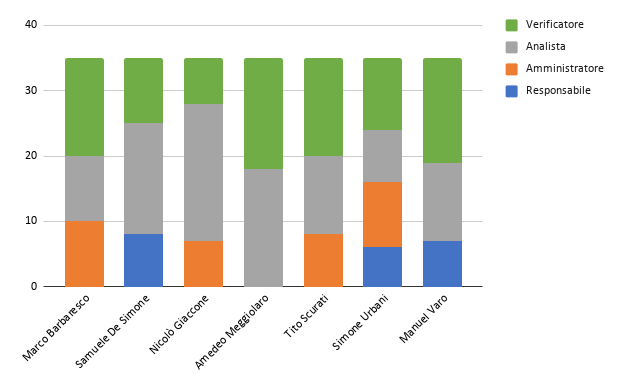
\includegraphics[scale=0.6]{../../../Images/Diagrammi/Istogrammi/ore analisi.png}
    \centering
    \caption{Istogramma della suddivisione delle ore per ruolo nell' Analisi}
\end{figure}
\subsubsection{Prospetto economico}
In questa fase i costi da affrontare per ogni ruolo sono i seguenti:
\begin{center}
    \begin{table}[ht!]
        \centering
        \caption{Prospetto dei costi per ruolo nel periodo di Analisi}
        \vspace{5px}
        \rowcolors{2}{logo!10}{logo!40}
        \renewcommand{\arraystretch}{1.8}
        \begin{tabular}{p{75px} p{20px} p{50px} }
            \rowcolor{logo!70} \textbf{Ruolo} & \textbf{Ore} & \textbf{Costo}  \\
            Responsabile                      & 21           & 630,00\EURdig   \\
            Amministratore                    & 35           & 700,00\EURdig   \\
            Analista                          & 98           & 2.450,00\EURdig \\
            Progettista                       & -            & -               \\
            Programmatore                     & -            & -               \\
            Verificatore                      & 91           & 1.365,00\EURdig \\
            Totale                            & 245          & 5.145,00\EURdig \\
        \end{tabular}
    \end{table}
\end{center}
\pagebreak
I dati appena descritti si possono riassumere nel seguente areogramma:
\begin{figure}[!h]
    \vspace{5px}
    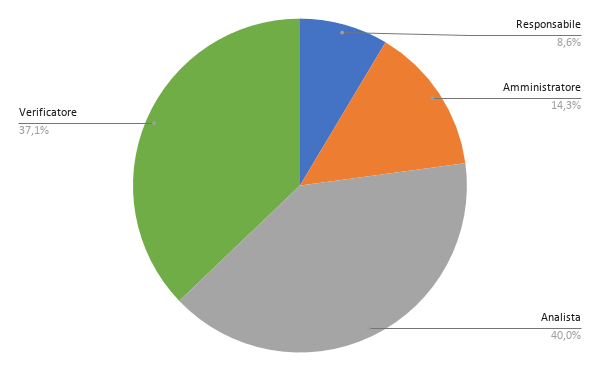
\includegraphics[scale=0.5]{../../../Images/Diagrammi/Diagramma a torta/ore analisi.png}
    \centering
    \caption{Areogramma della suddivisione di ore per ruolo in Analisi}
\end{figure}


\subsection{Fase di Consolidamento dei requisiti}
\subsubsection{Prospetto orario}
Per il periodo di Consolidamento dei requisiti la suddivisione oraria dei ruoli sarà la seguente:

\begin{center}
    \begin{table}[ht!]
        \centering
        \caption{Distribuzione delle ore della fase di Consolidamento dei requisiti}
        \vspace{5px}
        \rowcolors{2}{logo!10}{logo!40}
        \renewcommand{\arraystretch}{1.8}
        \begin{tabular}{p{100px} p{20px} p{20px} p{20px} p{20px} p{20px} p{20px} p{50px} }
            \rowcolor{logo!70} \textbf{Nominativo} & \textbf{Re} & \textbf{Am} & \textbf{An} & \textbf{Pt} & \textbf{Pr} & \textbf{Ve} & \textbf{Ore totali} \\
            Marco Barbaresco                       & -           & -           & 2           & -           & -           & 4           & 6                   \\
            Samuele De Simone                      & 4           & -           & -           & -           & -           & 2           & 6                   \\
            Nicolò Giaccone                        & -           & -           & 6           & -           & -           & -           & 6                   \\
            Amedeo Meggiolaro                      & -           & -           & -           & -           & -           & 6           & 6                   \\
            Tito Scutari                           & -           & -           & 6           & -           & -           & -           & 6                   \\
            Simone Urbani                          & -           & 6           & -           & -           & -           & -           & 6                   \\
            Manuel Varo                            & -           & -           & 2           & -           & -           & 4           & 6                   \\
            Ore totali di ruolo                    & 4           & 6           & 16          & -           & -           & 16          & 42                  \\
        \end{tabular}
    \end{table}
\end{center}
\pagebreak

I dati appena descritti si possono riassumere nel seguente istogramma:
\begin{figure}[!h]
    \vspace{5px}
    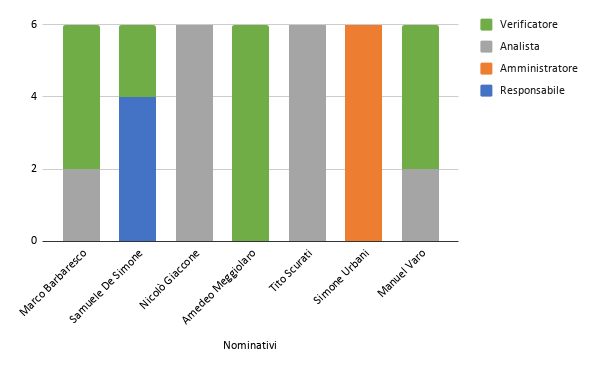
\includegraphics[scale=0.6]{../../../Images/Diagrammi/Istogrammi/ore requisiti.png}
    \centering
    \caption{Istogramma della ripartizione di ore per ruolo in Consolidamento dei requisiti}
\end{figure}

\subsubsection{Prospetto economico}
In questa fase i costi da affrontare per ogni ruolo sono i seguenti:
\begin{center}
    \begin{table}[ht!]
        \centering
        \caption{Prospetto dei costi per ruolo della fase di Consolidamento dei requisiti}
        \vspace{5px}
        \rowcolors{2}{logo!10}{logo!40}
        \renewcommand{\arraystretch}{1.8}
        \begin{tabular}{p{75px} p{20px} p{50px}}
            \rowcolor{logo!70} \textbf{Ruolo} & \textbf{Ore} & \textbf{Costo} \\
            Responsabile                      & 4            & 120,00\EURdig  \\
            Amministratore                    & 6            & 120,00\EURdig  \\
            Analista                          & 16           & 400,00\EURdig  \\
            Progettista                       & -            & -              \\
            Programmatore                     & -            & -              \\
            Verificatore                      & 16           & 240,00\EURdig  \\
            Totale                            & 42           & 880,00\EURdig  \\
        \end{tabular}
    \end{table}
\end{center}
\pagebreak

I dati appena descritti si possono riassumere nel seguente areogramma:
\begin{figure}[!h]
    \vspace{5px}
    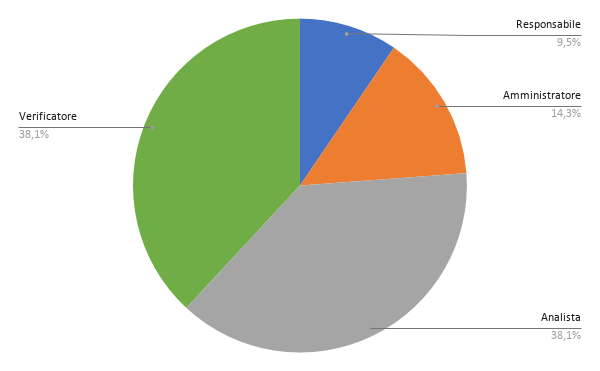
\includegraphics[scale=0.5]{../../../Images/Diagrammi/Diagramma a torta/ore requisiti.png}
    \centering
    \caption{Areogramma della ripartizione di ore per ruolo in Consolidamento dei requisiti}
\end{figure}



\subsection{Fase di Progettazione architetturale}
\subsubsection{Prospetto orario}
Durante il periodo di Progettazione architetturale la ripartizione oraria dei ruoli sarà la seguente:
\begin{center}
    \begin{table}[ht!]
        \centering
        \caption{Distribuzione delle ore della fase di Progettazione architetturale}
        \vspace{5px}
        \rowcolors{2}{logo!10}{logo!40}
        \renewcommand{\arraystretch}{1.8}
        \begin{tabular}{p{100px} p{20px} p{20px} p{20px} p{20px} p{20px} p{20px} p{50px} }
            \rowcolor{logo!70} \textbf{Nominativo} & \textbf{Re} & \textbf{Am} & \textbf{An} & \textbf{Pt} & \textbf{Pr} & \textbf{Ve} & \textbf{Ore totali} \\
            Marco Barbaresco                       & -           & -           & 6           & 13          & 5           & 4           & 28                  \\
            Samuele De Simone                      & -           & -           & 10          & -           & 6           & 12          & 28                  \\
            Nicolò Giaccone                        & -           & 7           & -           & 15          & 6           & -           & 28                  \\
            Amedeo Meggiolaro                      & 5           & -           & -           & 12          & 3           & 8           & 28                  \\
            Tito Scutari                           & 10          & 7           & -           & 11          & -           & -           & 28                  \\
            Simone Urbani                          & -           & -           & 6           & 12          & -           & 10          & 28                  \\
            Manuel Varo                            & -           & 5           & 8           & -           & 6           & 9           & 28                  \\
            Ore totali di ruolo                    & 15          & 19          & 30          & 63          & 26          & 43          & 196                 \\
        \end{tabular}
    \end{table}
\end{center}
\pagebreak

I dati appena descritti si possono riassumere nel seguente istogramma:
\begin{figure}[!h]
    \vspace{5px}
    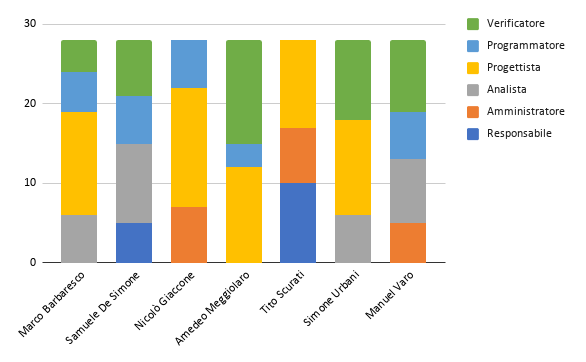
\includegraphics[scale=0.6]{../../../Images/Diagrammi/Istogrammi/ore architettura.png}
    \centering
    \caption{Istogramma della suddivisione di ore per ruolo in Progettazione architetturale}
\end{figure}

\subsubsection{Prospetto economico}
In questa fase i costi da affrontare per ogni ruolo sono i seguenti:
\begin{center}
    \begin{table}[ht!]
        \centering
        \caption{Prospetto dei costi per ruolo della fase di Progettazione architetturale}
        \vspace{5px}
        \rowcolors{2}{logo!10}{logo!40}
        \renewcommand{\arraystretch}{1.8}
        \begin{tabular}{p{75px} p{20px} p{50px}}
            \rowcolor{logo!70} \textbf{Ruolo} & \textbf{Ore} & \textbf{Costo}  \\
            Responsabile                      & 15           & 450,00\EURdig   \\
            Amministratore                    & 19           & 380,00\EURdig   \\
            Analista                          & 30           & 750,00\EURdig   \\
            Progettista                       & 63           & 1.368,00\EURdig \\
            Programmatore                     & 26           & 390,00\EURdig   \\
            Verificatore                      & 43           & 645,00\EURdig   \\
            Totale                            & 196          & 4.001,00\EURdig \\
        \end{tabular}
    \end{table}
\end{center}
\pagebreak

I dati appena descritti si possono riassumere nel seguente areogramma:
\begin{figure}[!h]
    \vspace{5px}
    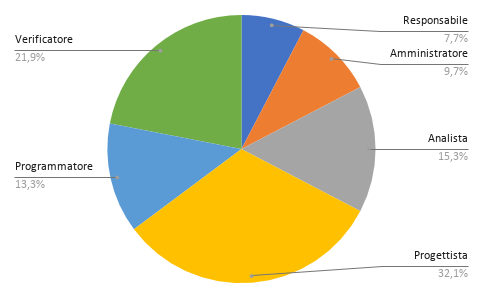
\includegraphics[scale=0.5]{../../../Images/Diagrammi/Diagramma a torta/ore architettura.png}
    \centering
    \caption{Areogramma della suddivisione di ore per ruolo in Progettazione architetturale}
\end{figure}


\subsection{Fase di Progettazione di dettaglio e codifica}
\subsubsection{Prospetto orario}
Per il periodo di Progettazione di dettaglio e codifica la ripartizione oraria dei ruoli sarà la seguente:
\begin{center}
    \begin{table}[ht!]
        \centering
        \caption{Distribuzione delle ore della fase di Progettazione di dettaglio e codifica}
        \vspace{5px}
        \rowcolors{2}{logo!10}{logo!40}
        \renewcommand{\arraystretch}{1.8}
        \begin{tabular}{p{100px} p{20px} p{20px} p{20px} p{20px} p{20px} p{20px} p{50px} }
            \rowcolor{logo!70} \textbf{Nominativo} & \textbf{Re} & \textbf{Am} & \textbf{An} & \textbf{Pt} & \textbf{Pr} & \textbf{Ve} & \textbf{Ore totali} \\
            Marco Barbaresco                       & 9           & -           & -           & 14          & 12          & 15          & 50                  \\
            Samuele De Simone                      & -           & 8           & -           & 18          & 13          & 11          & 50                  \\
            Nicolò Giaccone                        & 8           & -           & -           & 8           & 20          & 14          & 50                  \\
            Amedeo Meggiolaro                      & 6           & 5           & -           & 9           & 12          & 18          & 50                  \\
            Tito Scutari                           & -           & 9           & -           & 14          & 18          & 9           & 50                  \\
            Simone Urbani                          & 8           & -           & -           & 14          & 16          & 12          & 50                  \\
            Manuel Varo                            & -           & 12          & -           & 13          & 9           & 16          & 50                  \\
            Ore totali di ruolo                    & 31          & 34          & 0           & 90          & 100         & 95          & 350                 \\
        \end{tabular}
    \end{table}
\end{center}
\pagebreak

I dati appena descritti si possono riassumere nel seguente istogramma:
\begin{figure}[!h]
    \vspace{5px}
    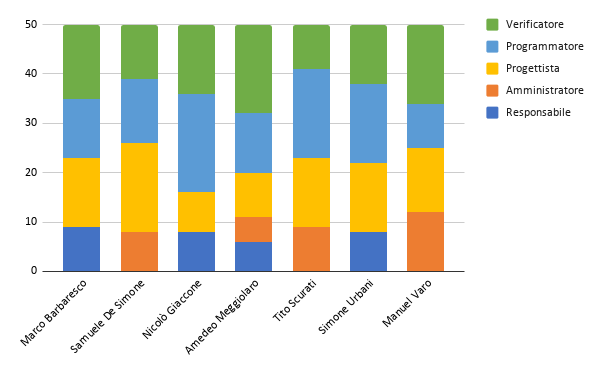
\includegraphics[scale=0.6]{../../../Images/Diagrammi/Istogrammi/ore codifica.png}
    \centering
    \caption{Istogramma della suddivisione di ore per ruolo in Progettazione di dettaglio e codifica}
\end{figure}
\subsubsection{Prospetto economico}
In questa fase i costi da affrontare per ogni ruolo sono i seguenti:
\begin{center}
    \begin{table}[ht!]
        \centering
        \caption{Prospetto dei costi per ruolo della fase di Progettazione di dettaglio e codifica}
        \vspace{5px}
        \rowcolors{2}{logo!10}{logo!40}
        \renewcommand{\arraystretch}{1.8}
        \begin{tabular}{p{75px} p{20px} p{50px}}
            \rowcolor{logo!70} \textbf{Ruolo} & \textbf{Ore} & \textbf{Costo}  \\
            Responsabile                      & 31           & 930,00\EURdig   \\
            Amministratore                    & 34           & 680,00\EURdig   \\
            Analista                          & -            & -               \\
            Progettista                       & 90           & 1.980,00\EURdig \\
            Programmatore                     & 100          & 1.500,00\EURdig \\
            Verificatore                      & 95           & 1.425,00\EURdig \\
            Totale                            & 350          & 6.515,00\EURdig \\
        \end{tabular}
    \end{table}
\end{center}
\pagebreak

I dati appena descritti si possono riassumere nel seguente areogramma:
\begin{figure}[!h]
    \vspace{5px}
    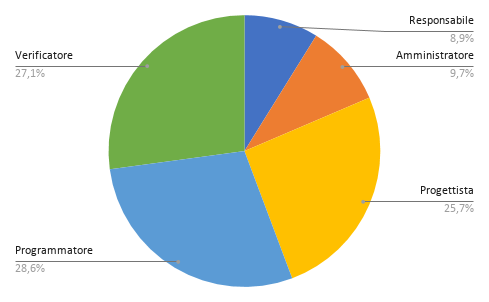
\includegraphics[scale=0.5]{../../../Images/Diagrammi/Diagramma a torta/ore codifica.png}
    \centering
    \caption{Areogramma della suddivisione di ore per ruolo in Progettazione di dettaglio e codifica}
\end{figure}



\subsection{Fase di Validazione e collaudo}
\subsubsection{Prospetto orario}
Per il periodo di Validazione e collaudo la ripartizione oraria dei ruoli sarà la seguente:
\begin{center}
    \begin{table}[ht!]
        \centering
        \caption{Distribuzione delle ore della fase di Validazione e collaudo}
        \vspace{5px}
        \rowcolors{2}{logo!10}{logo!40}
        \renewcommand{\arraystretch}{1.8}
        \begin{tabular}{p{100px} p{20px} p{20px} p{20px} p{20px} p{20px} p{20px} p{50px} }
            \rowcolor{logo!70} \textbf{Nominativo} & \textbf{Re} & \textbf{Am} & \textbf{An} & \textbf{Pt} & \textbf{Pr} & \textbf{Ve} & \textbf{Ore totali} \\
            Marco Barbaresco                       & -           & 8           & -           & 2           & -           & 10          & 20                  \\
            Samuele De Simone                      & 4           & -           & -           & -           & 7           & 9           & 20                  \\
            Nicolò Giaccone                        & -           & 5           & -           & 6           & -           & 9           & 20                  \\
            Amedeo Meggiolaro                      & -           & -           & -           & 12          & 8           & -           & 20                  \\
            Tito Scutari                           & 6           & -           & -           & -           & 12          & 2           & 20                  \\
            Simone Urbani                          & -           & 6           & -           & -           & 10          & 4           & 20                  \\
            Manuel Varo                            & 10          & -           & -           & -           & 4           & 6           & 20                  \\
            Ore totali di ruolo                    & 20          & 19          & 0           & 20          & 41          & 40          & 140                 \\
        \end{tabular}
    \end{table}
\end{center}
\pagebreak

I dati appena descritti si possono riassumere nel seguente istogramma:
\begin{figure}[!h]
    \vspace{5px}
    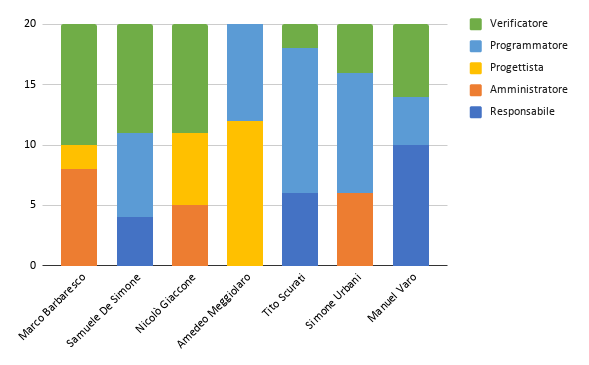
\includegraphics[scale=0.6]{../../../Images/Diagrammi/Istogrammi/ore validificazione.png}
    \centering
    \caption{Istogramma della suddivisione di ore per ruolo in Validazione e collaudo}
\end{figure}
\subsubsection{Prospetto economico}
In questa fase i costi da affrontare per ogni ruolo sono i seguenti:

\begin{center}
    \begin{table}[ht!]
        \centering
        \caption{Prospetto dei costi per ruolo della fase di Validazione e collaudo}
        \vspace{5px}
        \rowcolors{2}{logo!10}{logo!40}
        \renewcommand{\arraystretch}{1.8}
        \begin{tabular}{p{75px} p{20px} p{50px}}
            \rowcolor{logo!70} \textbf{Ruolo} & \textbf{Ore} & \textbf{Costo}  \\
            Responsabile                      & 20           & 600,00\EURdig   \\
            Amministratore                    & 19           & 380,00\EURdig   \\
            Analista                          & -            & -               \\
            Progettista                       & 20           & 440,00\EURdig   \\
            Programmatore                     & 41           & 615,00\EURdig   \\
            Verificatore                      & 40           & 600,00\EURdig   \\
            Totale                            & 140          & 2.635,00\EURdig \\
        \end{tabular}
    \end{table}
\end{center}
\pagebreak

I dati appena descritti si possono riassumere nel seguente areogramma:
\begin{figure}[!h]
    \vspace{5px}
    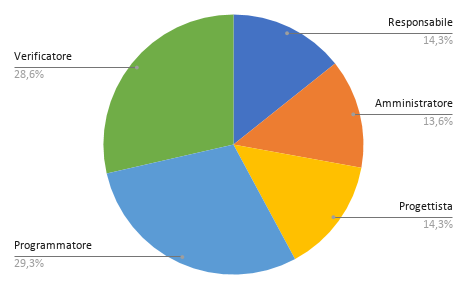
\includegraphics[scale=0.5]{../../../Images/Diagrammi/Diagramma a torta/ore validificazione.png}
    \centering
    \caption{Areogramma della suddivisione di ore per ruolo in Validazione e collaudo}
\end{figure}


\subsection{Riepilogo}
\subsubsection{Ore totali}
\subsubsubsection{Suddivisione lavoro}
Nella tabella sottostante è riportato il totale delle ore del progetto, sono presenti sia le ore d'investimento che quelle rendicontate a carico del committente:
\begin{center}
    \begin{table}[ht!]
        \centering\caption{Distribuzione delle ore totali d'investimento e rendicontate}
        \vspace{5px}
        \rowcolors{2}{logo!10}{logo!40}
        \renewcommand{\arraystretch}{1.8}
        \begin{tabular}{p{100px} p{20px} p{20px} p{20px} p{20px} p{20px} p{20px} p{50px} }
            \rowcolor{logo!70} \textbf{Nominativo} & \textbf{Re} & \textbf{Am} & \textbf{An} & \textbf{Pt} & \textbf{Pr} & \textbf{Ve} & \textbf{Ore totali} \\
            Marco Barbaresco                       & 9           & 18          & 18          & 29          & 17          & 48          & 139                 \\
            Samuele De Simone                      & 16          & 8           & 27          & 18          & 26          & 44          & 139                 \\
            Nicolò Giaccone                        & 8           & 19          & 27          & 29          & 26          & 30          & 139                 \\
            Amedeo Meggiolaro                      & 11          & 5           & 18          & 33          & 23          & 49          & 139                 \\
            Tito Scutari                           & 16          & 24          & 18          & 25          & 30          & 26          & 139                 \\
            Simone Urbani                          & 14          & 22          & 14          & 26          & 26          & 37          & 139                 \\
            Manuel Varo                            & 17          & 17          & 22          & 13          & 19          & 51          & 139                 \\
            Ore totali di ruolo                    & 91          & 113         & 144         & 173         & 167         & 285         & 973                 \\
        \end{tabular}
    \end{table}
\end{center}
\pagebreak
Una rappresentazione visiva della suddivisione oraria viene data dal seguente grafico:

\begin{figure}[!h]
    \vspace{5px}
    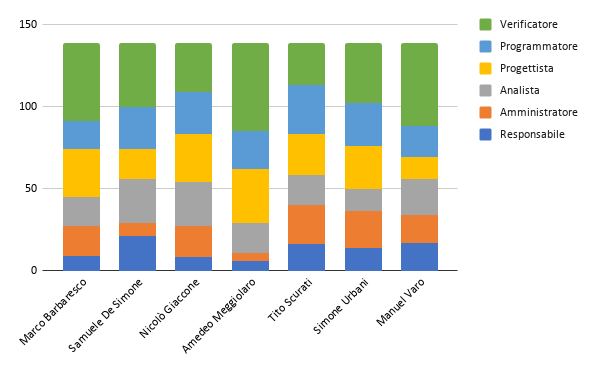
\includegraphics[scale=0.6]{../../../Images/Diagrammi/Istogrammi/ore totali.png}
    \centering
    \caption{Istogramma della suddivisione delle ore totali d'investimento e rendicontate}
\end{figure}

\subsubsubsection{Prospetto economico}
I costi da affrontare per ogni ruolo sono i seguenti:
\begin{center}
    \begin{table}[ht!]
        \centering
        \caption{Prospetto dei costi totale delle ore d'investimento e rendicontate}
        \vspace{5px}
        \rowcolors{2}{logo!10}{logo!40}
        \renewcommand{\arraystretch}{1.8}
        \begin{tabular}{p{75px} p{20px} p{50px}}
            \rowcolor{logo!70} \textbf{Ruolo} & \textbf{Ore} & \textbf{Costo}   \\
            Responsabile                      & 91           & 2.730,00\EURdig  \\
            Amministratore                    & 113          & 2.260,00\EURdig  \\
            Analista                          & 144          & 3.600,00\EURdig  \\
            Progettista                       & 173          & 3.806,00\EURdig  \\
            Programmatore                     & 167          & 2.505,00\EURdig  \\
            Verificatore                      & 285          & 4.275,00\EURdig  \\
            Totale                            & 973          & 19.176,00\EURdig \\
        \end{tabular}
    \end{table}
\end{center}
\pagebreak
dati ottenuti si possono riassumere nel seguente areogramma:
\begin{figure}[!h]
    \vspace{5px}
    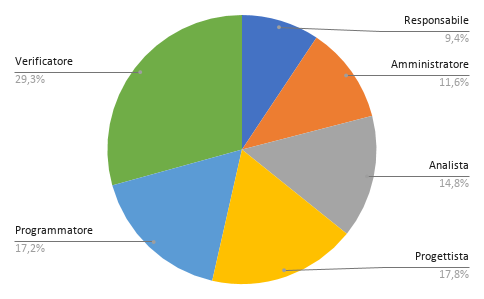
\includegraphics[scale=0.5]{../../../Images/Diagrammi/Diagramma a torta/ore totali.png}
    \centering
    \caption{Areogramma dei costi delle ore totali d'investimento e rendicontate}
\end{figure}

\subsubsection{Ore rendicontate}
\subsubsubsection{Suddivisione lavoro}
Le ore rendicontate sono riportate nella seguente tabella:
\begin{center}
    \begin{table}[ht!]
        \centering
        \caption{Distribuzione delle ore rendicontate}
        \vspace{5px}
        \rowcolors{2}{logo!10}{logo!40}
        \renewcommand{\arraystretch}{1.8}
        \begin{tabular}{p{100px} p{20px} p{20px} p{20px} p{20px} p{20px} p{20px} p{50px} }
            \rowcolor{logo!70} \textbf{Nominativo} & \textbf{Re} & \textbf{Am} & \textbf{An} & \textbf{Pt} & \textbf{Pr} & \textbf{Ve} & \textbf{Ore totali} \\
            Marco Barbaresco                       & 9           & 8           & 8           & 29          & 17          & 33          & 104                 \\
            Samuele De Simone                      & 8           & 8           & 10          & 18          & 26          & 34          & 104                 \\
            Nicolò Giaccone                        & 8           & 12          & 6           & 29          & 26          & 23          & 104                 \\
            Amedeo Meggiolaro                      & 11          & 5           & 0           & 33          & 23          & 32          & 104                 \\
            Tito Scutari                           & 16          & 16          & 6           & 25          & 30          & 11          & 104                 \\
            Simone Urbani                          & 8           & 12          & 6           & 26          & 26          & 26          & 104                 \\
            Manuel Varo                            & 10          & 17          & 10          & 13          & 19          & 35          & 104                 \\
            Ore totali di ruolo                    & 70          & 78          & 46          & 173         & 167         & 194         & 728                 \\
        \end{tabular}
    \end{table}
\end{center}
\pagebreak
Una rappresentazione visiva della suddivisione oraria viene data dal seguente grafico:
\begin{figure}[!h]
    \vspace{5px}
    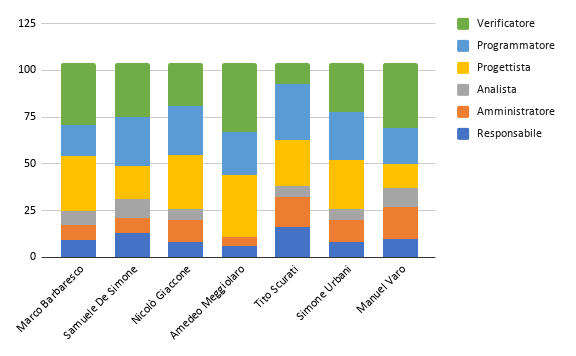
\includegraphics[scale=0.6]{../../../Images/Diagrammi/Istogrammi/ore rendicontate.png}
    \centering
    \caption{Istogramma della suddivisione delle ore rendicontate}
\end{figure}

\subsubsubsection{Prospetto economico}
Il totale rendicontato dei costi da affrontare per ogni ruolo è:

\begin{center}
    \begin{table}[ht!]
        \centering
        \caption{Prospetto dei costi delle ore rendicontate}
        \vspace{5px}
        \rowcolors{2}{logo!10}{logo!40}
        \renewcommand{\arraystretch}{1.8}
        \begin{tabular}{p{75px} p{20px} p{50px}}
            \rowcolor{logo!70} \textbf{Ruolo} & \textbf{Ore} & \textbf{Costo}   \\
            Responsabile                      & 70           & 2.100,00\EURdig  \\
            Amministratore                    & 78           & 1.560,00\EURdig  \\
            Analista                          & 46           & 1.150,00\EURdig  \\
            Progettista                       & 173          & 3.806,00\EURdig  \\
            Programmatore                     & 167          & 2.505,00\EURdig  \\
            Verificatore                      & 194          & 2.910,00\EURdig  \\
            Totale                            & 728          & 14.031,00\EURdig \\
        \end{tabular}
    \end{table}
\end{center}
\pagebreak
dati ottenuti si possono riassumere nel seguente areogramma:
\begin{figure}[!h]
    \vspace{5px}
    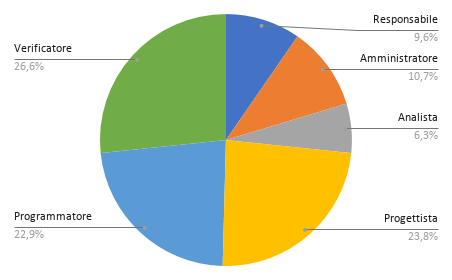
\includegraphics[scale=0.5]{../../../Images/Diagrammi/Diagramma a torta/ore rendicontate.png}
    \centering
    \caption{Areogramma delle ore rendicontate per ruolo}
\end{figure}

\subsection{Conclusioni}
Considerando solamente le ore rendicontate, il costo del progetto è di: 14.031,00\EURdig.
\section{Consuntivi di periodo}
Di seguito vengono indicate le spese sostenute per ogni ruolo confrontandole con quanto preventivato. Il bilancio potrà essere:
\begin{itemize}
    \item \textbf{Positivo:} se la spesa effettiva è minore di quanto preventivato;
    \item \textbf{Pari:} se la spesa effettiva è uguale a quanto preventivato;
    \item \textbf{Negativo:} se la spesa effettiva è maggiore di quanto preventivato.
\end{itemize}

\subsection{Periodo di analisi}
Le ore di lavoro sostenute in questa fase sono da considerarsi come ore d'investimento per l'approfondimento personale, non vengono quindi rendicontate.

\begin{center}
    \begin{table}[!ht]
        \centering
        \caption{Consuntivo della fase di analisi}
        \vspace{5px}
        \rowcolors{2}{logo!10}{logo!40}
        \renewcommand{\arraystretch}{1.8}
        \begin{tabular}{p{150px} p{110px} p{110px}}
            \rowcolor{logo!70} \textbf{Ruolo} & \textbf{Ore} & \textbf{Costo}                  \\
            Responsabile                      & 21 (+0)      & 630,00\EURdig (+0,00 \EURdig)   \\
            Amministratore                    & 35 (+0)      & 700,00\EURdig (+0,00 \EURdig)   \\
            Analista                          & 98 (+0)      & 2.450,00\EURdig (+0,00 \EURdig) \\
            Progettista                       & 0 (+0)       & 0(+0,00 \EURdig)                \\
            Programmatore                     & 0 (+0)       & 0(+0,00 \EURdig)                \\
            Verificatore                      & 91 (+0)      & 1.365,00\EURdig (+0,00 \EURdig) \\
            \textbf{Totale preventivo}        & 245          & 5.145,00\EURdig                 \\
            \textbf{Totale consuntivo}        & 245          & 5.145,00\EURdig                 \\
            \textbf{Differenza}               & 0            & (+0,00 \EURdig)                 \\
        \end{tabular}
    \end{table}
\end{center}
\subsubsection{Conclusioni}
Avendo deciso con i componenti del gruppo di rispettare la scadenza per la prima consegna disponibile, si è lavorato per rispettare i tempi e si è riusciti a non superare le tempistiche prestabilite.

\subsubsection{Preventivo a finire}
Rispettando le tempistiche preventivate non sono stati aggiunti costi alla fase di analisi.

\newpage
\subsection{Periodo di Consolidamento dei requisiti}
In questo periodo si è svolto il lavoro relativo al consolidamento dei requisiti, successivo a quello di analisi. Sono state dedicate delle ore anche per lo studio e l'approfondimento personale e sono da considerarsi come non rendicontate. Perciò tali ore non sono state riportate nella seguente tabella:

\begin{center}
    \begin{table}[ht!]
        \centering
        \caption{Consuntivo della fase di Consolidamento dei requisiti}
        \vspace{5px}
        \rowcolors{2}{logo!10}{logo!40}
        \renewcommand{\arraystretch}{1.8}
        \begin{tabular}{p{150px} p{110px} p{110px}}
            \rowcolor{logo!70} \textbf{Ruolo} & \textbf{Ore} & \textbf{Costo}                 \\
            Responsabile                      & 5 (+1)       & 150,00\EURdig (+30,00 \EURdig) \\
            Amministratore                    & 6 (+0)       & 120,00\EURdig (+0,00 \EURdig)  \\
            Analista                          & 13 (-3)      & 325,00\EURdig (-75,00 \EURdig) \\
            Progettista                       & 0 (+0)       & 0 (+0,00 \EURdig)              \\
            Programmatore                     & 0 (+0)       & 0 (+0,00 \EURdig)              \\
            Verificatore                      & 16 (+0)      & 240,00\EURdig (+0,00 \EURdig)  \\
            \textbf{Totale preventivo}        & 42           & 880,00\EURdig                  \\
            \textbf{Totale consuntivo}        & 40           & 835,00\EURdig                  \\
            \textbf{Differenza}               & -2           & (-45,00\EURdig)                \\
        \end{tabular}
    \end{table}
\end{center}

\subsubsection{Conclusioni}
Rispetto a quanto preventivato inizialmente sono state necessarie delle modifiche per il lavoro svolto durante questo periodo. Vista la ridotta durata di tale periodo il gruppo è riuscito a ridurre le ore necessarie al completamento del lavoro. Di seguito sono riportate le motivazioni delle variazioni del monte ore di lavoro ricoperto dai diversi ruoli:
\begin{itemize}
    \item \textbf{\textit{Responsabile}} è stata necessaria un'ora aggiuntiva, per la coordinazione dei membri del gruppo inerente alla presentazione e allo studio delle tecnologie, necessarie allo sviluppo software;
    \item \textbf{\textit{Analista}} Viste le non eccessive modifiche nella documentazione sono state necessarie meno ore in questo ruolo.
\end{itemize}

\subsubsection{Preventivo a finire} Il bilancio economico risultante è positivo, ovvero sono stati risparmiati 45,00\EURdig. Tali fondi verranno impiegati nei prossimi periodi per far fronte a eventuali ritardi.

\newpage
\subsection{Periodo di Progettazione architetturale}
Le ore sostenute durante questo periodo sono relative alla progettazione e alla codifica del \textit{Proof of Concept}\textsubscript{\textbf{G}}, necessario al soddisfacimento della \textit{Technology Baseline}\textsubscript{\textbf{G}}. Tale periodo è da considerarsi rendicontato, in quanto il capitolato d'appalto è stato aggiudicato e quindi il lavoro è svolto con lo scopo di sviluppare il prodotto finale.

\begin{center}
    \begin{table}[ht!]
        \centering
        \caption{Consuntivo dei costi per ruolo della fase di Progettazione architetturale}
        \vspace{5px}
        \rowcolors{2}{logo!10}{logo!40}
        \renewcommand{\arraystretch}{1.8}
        \begin{tabular}{p{150px} p{110px} p{110px}}
            \rowcolor{logo!70} \textbf{Ruolo} & \textbf{Ore} & \textbf{Costo}                 \\
            Responsabile                      & 15(+0)       & 450,00\EURdig(+0,00 \EURdig)   \\
            Amministratore                    & 22(+3)       & 440,00\EURdig(+60,00 \EURdig)  \\
            Analista                          & 28(-2)       & 700,00\EURdig(-50,00 \EURdig)  \\
            Progettista                       & 41(-22)      & 902,00\EURdig(-484,00 \EURdig) \\
            Programmatore                     & 50(+24)      & 750,00\EURdig(+360,00 \EURdig) \\
            Verificatore                      & 43(+0)       & 645,00\EURdig(+0,00 \EURdig)   \\
            \textbf{Totale preventivo}        & 196          & 4001,00\EURdig                 \\
            \textbf{Totale consuntivo}        & 199          & 3887,00\EURdig                 \\
            \textbf{Differenza}               & +3           & (-114,00 \EURdig)              \\
        \end{tabular}
    \end{table}
\end{center}

\subsubsection{Conclusioni}
Dai dati riportati nella tabella soprastante si può notare che la progettazione riguardante tale periodo ha subito una consistente modifica. Il gruppo aveva infatti pianificato di redigere una completa progettazione architetturale del prodotto, e di riportarla all’ interno di un documento formale. Tuttavia durante lo svolgimento del lavoro ci si è concentrati maggiormente sul verificare, attraverso la progettazione e la codifica del \textit{Proof of Concept}\textsubscript{\textbf{G}}, che le tecnologie scelte si integrassero efficientemente tra loro, e che con il loro utilizzo i requisiti potessero essere soddisfatti. Di seguito sono riportate le motivazioni delle variazioni del monte ore di lavoro ricoperto dai diversi ruoli:

\begin{itemize}
    \item \textbf{\textit{Amministratore:}} Essendoci stata una maggiore necessità di sistemazione riguardante il versionamento dei documenti, si è presentato un esubero di ore per questo ruolo;
    \item \textbf{\textit{Analista:}} Vista una minore necessità di modifica riguardante la correzione dei casi d'uso e la fase di analisi per la risoluzione dei problemi, vi è stato un decremento delle ore riguardanti gli \textit{Analisti};
    \item \textbf{\textit{Progettista:}} Essendo state scelte preventivamente tutte le tecnologie da parte dei proponenti, non è servito un grande dispendio di ore per la scelta delle stesse;
    \item \textbf{\textit{Programmatore:}} Essendo stato implementato il \textit{Proof of Concept} collegando tutte le tecnologie essenziali allo sviluppo del progetto, si è reso necessario un maggiore dispendio di ore per poter collegare tutte le tecnologie previste.
\end{itemize}

Le ore di lavoro riguardanti ai ruoli che hanno subito delle variazioni rispetto a quanto pianificato sono state distribuite in modo tale che ogni elemento del gruppo svolgesse lo stesso monte ore di lavoro complessivo.

\subsubsection{Preventivo a finire} Il bilancio economico risultante è positivo, ovvero sono stati risparmiati 114,00\EURdig. Tali fondi uniti a quelli già risparmiati nel periodo precedente, per un totale di 159,00\EurDig, saranno impiegati nei prossimi periodi per far fronte a eventuali ritardi o per implementare i requisiti opzionali.


\newpage
\subsection{Periodo di Progettazione di dettaglio e codifica}
\subsubsection{Incremento 6}
\begin{center}
    \begin{table}[ht!]
        \centering
        \caption{Consuntivo dei costi per ruolo dell'incremento 6}
        \vspace{5px}
        \rowcolors{2}{logo!10}{logo!40}
        \renewcommand{\arraystretch}{1.8}
        \begin{tabular}{p{150px} p{110px} p{110px}}
            \rowcolor{logo!70} \textbf{Ruolo} & \textbf{Ore} & \textbf{Costo}                 \\
            Responsabile                      & 5(+0)        & 150,00\EURdig(+0,00 \EURdig)   \\
            Amministratore                    & 13(+4)       & 260,00\EURdig(+80,00 \EURdig)   \\
            Analista                          & 0(+0)        & 0,00\EURdig(+0,00 \EURdig)     \\
            Progettista                       & 30(+0)       & 660,00\EURdig(+0,00 \EURdig)   \\
            Programmatore                     & 0(+0)        & 0,00\EURdig(+0,00 \EURdig)     \\
            Verificatore                      & 12(+0)       & 180,00\EURdig(+0,00 \EURdig)   \\
            \textbf{Totale preventivo}        & 56           & 1.170,00\EURdig                \\
            \textbf{Totale consuntivo}        & 60           & 1.250,00\EURdig                \\
            \textbf{Differenza}               & +4           & (+80,00 \EURdig)                \\
        \end{tabular}
    \end{table}
\end{center}
\subsubsubsection{Conclusioni}
Avendo dovuto modificare in maniera più approfondita del previsto le \textit{Norme di Progetto}, si sono rese necessarie più ore di \textit{Amministratore} rispetto a quanto preventivato.
\subsubsubsection{Preventivo a finire rispetto alla fase}
L'aumento delle ore di \textit{Amministratore} ha portato ad un incremento del costo per un totale di 80,00 \EURdig.
\subsubsubsection{Preventivo a finire complessivo}
La spesa aggiuntiva, sottratta al risparmio accumulato nella fase precedente, mantiene comunque il bilancio positivo di 79,00\EurDig, che saranno impiegati nei prossimi periodi per far fronte a eventuali ritardi o per implementare i requisiti opzionali.

\pagebreak
\subsubsection{Incremento 7}
\begin{center}
    \begin{table}[ht!]
        \centering
        \caption{Consuntivo dei costi per ruolo dell'incremento 7}
        \vspace{5px}
        \rowcolors{2}{logo!10}{logo!40}
        \renewcommand{\arraystretch}{1.8}
        \begin{tabular}{p{150px} p{110px} p{110px}}
            \rowcolor{logo!70} \textbf{Ruolo} & \textbf{Ore}  & \textbf{Costo}                     \\
            Responsabile                      & 8(+2)         & 240,00\EURdig(+0,00 \EURdig)       \\
            Amministratore                    & 6(+0)         & 120,00\EURdig(+0,00 \EURdig)       \\
            Analista                          & 0(+0)         & 0,00\EURdig(+0,00 \EURdig)         \\
            Progettista                       & 20(-3)        & 440,00\EURdig(+0,00 \EURdig)       \\
            Programmatore                     & 10(+0)        & 150,00\EURdig(+0,00 \EURdig)       \\
            Verificatore                      & 11(+0)        & 165,00\EURdig(+0,00 \EURdig)       \\
            \textbf{Totale preventivo}        & 56            & 1.121,00\EURdig                    \\
            \textbf{Totale consuntivo}        & 55            & 1.115,00\EURdig                    \\
            \textbf{Differenza}               & -1            & (-6,00 \EURdig)                    \\
        \end{tabular}
    \end{table}
\end{center}
\subsubsubsection{Conclusioni}
A causa di imprevisti ed impegni personali dei membri del gruppo, sono risultate necessarie più ore di \textit{Responsabile} rispetto a quanto preventivato, per organizzare il lavoro dei componenti del gruppo in maniera efficiente. Avendo effettuato scelte ponderate riguardo alle tecnologie da utilizzare per lo sviluppo del progetto, in questo incremento sono risultate necessarie meno ore di \textit{Progettista} rispetto a quanto preventivato.
\subsubsubsection{Preventivo a finire rispetto alla fase}
La differenza tra le ore di \textit{Responsabile} Aggiunte e quelle di \textit{Progettista} rimosse ha portato ad un risparmio di 6,00 \EURdig in questo incremento.
\subsubsubsection{Preventivo a finire complessivo}
I soldi risparmiati, sommati a quelli risultanti alla fine dell'incremento precedente, portano ad un bilancio positivo di 85,00\EurDig, che saranno impiegati nei prossimi periodi per far fronte a eventuali ritardi o per implementare i requisiti opzionali.

\pagebreak
\subsubsection{Incremento 8}
\begin{center}
    \begin{table}[ht!]
        \centering
        \caption{Consuntivo dei costi per ruolo dell'incremento 8}
        \vspace{5px}
        \rowcolors{2}{logo!10}{logo!40}
        \renewcommand{\arraystretch}{1.8}
        \begin{tabular}{p{150px} p{110px} p{110px}}
            \rowcolor{logo!70} \textbf{Ruolo} & \textbf{Ore}  & \textbf{Costo}                    \\
            Responsabile                      & 3(+0)         & 90,00\EURdig(+0,00 \EURdig)       \\
            Amministratore                    & 5(+1)         & 100,00\EURdig(+0,00 \EURdig)      \\
            Analista                          & 0(+0)         & 0,00\EURdig(+0,00 \EURdig)        \\
            Progettista                       & 14(+0)        & 308,00\EURdig(+0,00 \EURdig)      \\
            Programmatore                     & 18(+5)        & 270,00\EURdig(+0,00 \EURdig)      \\
            Verificatore                      & 8(+0)         & 120,00\EURdig(+0,00 \EURdig)      \\
            \textbf{Totale preventivo}        & 42            & 793,00\EURdig                     \\
            \textbf{Totale consuntivo}        & 48            & 888,00\EURdig                     \\
            \textbf{Differenza}               & +6            & (+95,00 \EURdig)                  \\
        \end{tabular}
    \end{table}
\end{center}
\subsubsubsection{Conclusioni}
Avendo avuto difficoltà nella configurazione del linter \textit{Eslint} e con le modifiche apportate per la suddivisione dei repository in maniera più appropriata alla filosofia dei microservizi, si è presentato un esubero delle ore di \textit{Programmatore}. La conseguente modifica delle \textit{Norme di Progetto}, legata alla modifica della struttura dei repository e alla conseguente descrizione della nuova struttura, ha portato ad un esubero delle ore di \textit{Amministratore} rispetto a quanto preventivato.
\subsubsubsection{Preventivo a finire rispetto alla fase}
L'aumento delle ore di codifica ha portato ad un esubero di 75,00 \EURdig rispetto al bilancio dell'incremento.
\subsubsubsection{Preventivo a finire complessivo}
La spesa aggiuntiva, sottratta al risparmio accumulato negli incrementi precedenti, porta ad un bilancio negativo di -10,00\EurDig, questi soldi verranno recuperati con un'oculata gestione delle risorse.

\pagebreak
\subsubsection{Incremento 9}
\begin{center}
    \begin{table}[ht!]
        \centering
        \caption{Consuntivo dei costi per ruolo dell'incremento 9}
        \vspace{5px}
        \rowcolors{2}{logo!10}{logo!40}
        \renewcommand{\arraystretch}{1.8}
        \begin{tabular}{p{150px} p{110px} p{110px}}
            \rowcolor{logo!70} \textbf{Ruolo} & \textbf{Ore}  & \textbf{Costo}                   \\
            Responsabile                      & 2(+0)         & 60,00\EURdig(+0,00 \EURdig)      \\
            Amministratore                    & 2(+0)         & 40,00\EURdig(+0,00 \EURdig)      \\
            Analista                          & 0(+0)         & 0,00\EURdig(+0,00 \EURdig)       \\
            Progettista                       & 10(+0)        & 220,00\EURdig(+0,00 \EURdig)     \\
            Programmatore                     & 8(+0)         & 120,00\EURdig(+0,00 \EURdig)     \\
            Verificatore                      & 6(+0)         & 90,00\EURdig(+0,00 \EURdig)      \\
            \textbf{Totale preventivo}        & 28            & 530,00\EURdig                    \\
            \textbf{Totale consuntivo}        & 28            & 530,00\EURdig                    \\
            \textbf{Differenza}               & +0            & (+0,00\EURdig)                   \\
        \end{tabular}
    \end{table}
\end{center}
\subsubsubsection{Conclusioni}
Durante questo incremento è stato rispettato il numero di ore disponibili come risorse per implementare gli obiettivi, questo ha portato in pari le spese da sostenere rispetto a quanto preventivato.
\subsubsubsection{Preventivo a finire rispetto alla fase}
Tutti gli obiettivi dell’incremento sono stati raggiunti con successo, nel pieno rispetto del consumo di risorse preventivato. Il bilancio dell’incremento è quindi in pari.
\subsubsubsection{Preventivo a finire complessivo}
Date le considerazioni precedenti su costi e obiettivi, il preventivo complessivo resta invariato.

\pagebreak
\subsubsection{Incremento 10}
\begin{center}
    \begin{table}[ht!]
        \centering
        \caption{Consuntivo dei costi per ruolo dell'incremento 10}
        \vspace{5px}
        \rowcolors{2}{logo!10}{logo!40}
        \renewcommand{\arraystretch}{1.8}
        \begin{tabular}{p{150px} p{110px} p{110px}}
            \rowcolor{logo!70} \textbf{Ruolo} & \textbf{Ore}  & \textbf{Costo}                   \\
            Responsabile                      & 4(+0)         & 120,00\EURdig(+0,00 \EURdig)     \\
            Amministratore                    & 3(+0)         & 60,00\EURdig(+0,00 \EURdig)      \\
            Analista                          & 0(+0)         & 0,00\EURdig(+0,00 \EURdig)       \\
            Progettista                       & 3(+0)         & 66,00\EURdig(+0,00 \EURdig)      \\
            Programmatore                     & 22(+3)        & 285,00\EURdig(+0,00 \EURdig)     \\
            Verificatore                      & 9(-4)         & 195,00\EURdig(+0,00 \EURdig)     \\
            \textbf{Totale preventivo}        & 42            & 726,00\EURdig                    \\
            \textbf{Totale consuntivo}        & 41            & 711,00\EURdig                    \\
            \textbf{Differenza}               & -1            & (-15,00 \EURdig)                 \\
        \end{tabular}
    \end{table}
\end{center}
\subsubsubsection{Conclusioni}
Avendo avuto dei problemi con l'implementazione del carrello e del checkout nell’integrazione tra lambda e struttura dei servizi, si sono rese necessarie più ore di \textit{Programmatore} rispetto a quanto preventivato. La minor necessità di verifica dei documenti rispetto a quanto previsto ha portato ad un calo delle ore di \textit{Verificatore}.
\subsubsubsection{Preventivo a finire rispetto alla fase}
L'aggiunta delle ore di \textit{Programmatore} sottratte a quelle da \textit{Verificatore} portano ad un risparmio durante la fase di 15,00\EurDig.
\subsubsubsection{Preventivo a finire complessivo}
i 15,00\EurDig risparmiati, sottratti sommati alla spesa in esubero di 10,00\EurDig, porta il bilancio in positivo di 5,00\EurDig, che saranno impiegati nei prossimi periodi per far fronte a eventuali ritardi o per implementare i requisiti opzionali.

\pagebreak
\subsubsection{Incremento 11}
\begin{center}
    \begin{table}[ht!]
        \centering
        \caption{Consuntivo dei costi per ruolo dell'incremento 11}
        \vspace{5px}
        \rowcolors{2}{logo!10}{logo!40}
        \renewcommand{\arraystretch}{1.8}
        \begin{tabular}{p{150px} p{110px} p{110px}}
            \rowcolor{logo!70} \textbf{Ruolo} & \textbf{Ore}  & \textbf{Costo}                   \\
            Responsabile                      & 3(+0)         & 90,00\EURdig(+0,00 \EURdig)      \\
            Amministratore                    & 2(+0)         & 40,00\EURdig(+0,00 \EURdig)      \\
            Analista                          & 0(+0)         & 0,00\EURdig(+0,00 \EURdig)       \\
            Progettista                       & 4(+0)         & 88,00\EURdig(+0,00 \EURdig)      \\
            Programmatore                     & 14(+2)        & 180,00\EURdig(+0,00 \EURdig)     \\
            Verificatore                      & 7(+0)         & 105,00\EURdig(+0,00 \EURdig)     \\
            \textbf{Totale preventivo}        & 28            & 503,00\EURdig                    \\
            \textbf{Totale consuntivo}        & 30            & 533,00\EURdig                    \\
            \textbf{Differenza}               & +2            & (+30,00 \EURdig)                  \\
        \end{tabular}
    \end{table}
\end{center}
\subsubsubsection{Conclusioni}
Dopo aver parlato coi proponenti si è deciso di implementare le tecnologie \textit{SNS} ed \textit{SQS}, questo ha portato ad un incremento delle ore di \textit{Programmatore} necessarie.
\subsubsubsection{Preventivo a finire rispetto alla fase}
L'aggiunta delle ore di \textit{Programmatore} ha portato ad un aumento dei costi durante l'incremento di 30,00\EurDig.
\subsubsubsection{Preventivo a finire complessivo}
La spesa aggiuntiva porta ad un bilancio negativo di -25,00\EurDig, questi soldi verranno recuperati con un'oculata gestione delle risorse.

\pagebreak
\subsubsection{Incremento 12}
\begin{center}
    \begin{table}[ht!]
        \centering
        \caption{Consuntivo dei costi per ruolo dell'incremento 12}
        \vspace{5px}
        \rowcolors{2}{logo!10}{logo!40}
        \renewcommand{\arraystretch}{1.8}
        \begin{tabular}{p{150px} p{110px} p{110px}}
            \rowcolor{logo!70} \textbf{Ruolo} & \textbf{Ore}  & \textbf{Costo}                   \\
            Responsabile                      & 2(-1)         & 60,00\EURdig(+0,00 \EURdig)      \\
            Amministratore                    & 3(+0)         & 60,00\EURdig(+0,00 \EURdig)      \\
            Analista                          & 0(+0)         & 0,00\EURdig(+0,00 \EURdig)       \\
            Progettista                       & 6(+0)         & 132,00\EURdig(+0,00 \EURdig)     \\
            Programmatore                     & 15(+2)        & 225,00\EURdig(+0,00 \EURdig)     \\
            Verificatore                      & 17(+0)        & 255,00\EURdig(+0,00 \EURdig)     \\
            \textbf{Totale preventivo}        & 42            & 732,00\EURdig                    \\
            \textbf{Totale consuntivo}        & 43            & 732,00\EURdig                    \\
            \textbf{Differenza}               & +1            & (+0,00 \EURdig)                  \\
        \end{tabular}
    \end{table}
\end{center}
\subsubsubsection{Conclusioni}
Avendo avuto difficoltà nell'implementazione dei filtri dal lato frontend, si sono rese necessarie più ore di \textit{Programmatore} rispetto a quanto preventivato. Essendo stato organizzato precedentemente il lavoro, si è reso necessario meno tempo del previsto da responsabile.
\subsubsubsection{Preventivo a finire rispetto alla fase}
L'aggiunta delle ore di \textit{Programmatore} sottratte a quelle da \textit{Responsabile} portano in pari il costo del bilancio dell'incremento corrente.
\subsubsubsection{Preventivo a finire complessivo}
Date le considerazioni precedenti su costi e obiettivi, il preventivo complessivo resta invariato.

\pagebreak
\subsubsection{Incremento 13}
\begin{center}
    \begin{table}[ht!]
        \centering
        \caption{Consuntivo dei costi per ruolo dell'incremento 13}
        \vspace{5px}
        \rowcolors{2}{logo!10}{logo!40}
        \renewcommand{\arraystretch}{1.8}
        \begin{tabular}{p{150px} p{110px} p{110px}}
            \rowcolor{logo!70} \textbf{Ruolo} & \textbf{Ore}  & \textbf{Costo}                   \\
            Responsabile                      & 5(+0)         & 150,00\EURdig(+0,00 \EURdig)     \\
            Amministratore                    & 5(+0)         & 100,00\EURdig(+0,00 \EURdig)     \\
            Analista                          & 0(+0)         & 0,00\EURdig(+0,00 \EURdig)       \\
            Progettista                       & 0(+0)         & 0,00\EURdig(+0,00 \EURdig)       \\
            Programmatore                     & 25(+0)        & 375,00\EURdig(+0,00 \EURdig)     \\
            Verificatore                      & 21(+0)        & 315,00\EURdig(+0,00 \EURdig)     \\
            \textbf{Totale preventivo}        & 56            & 940,00\EURdig                    \\
            \textbf{Totale consuntivo}        & 56            & 940,00\EURdig                    \\
            \textbf{Differenza}               & +0            & (+0,00 \EURdig)                  \\
        \end{tabular}
    \end{table}
\end{center}
\subsubsubsection{Conclusioni}
Durante questo incremento è stato rispettato il numero di ore disponibili come risorse per implementare gli obiettivi, questo ha portato in pari le spese da sostenere rispetto a quanto preventivato.
\subsubsubsection{Preventivo a finire rispetto alla fase}
Tutti gli obiettivi dell’incremento sono stati raggiunti con successo, nel pieno rispetto del consumo di risorse preventivato. Il bilancio dell’incremento è quindi in pari.
\subsubsubsection{Preventivo a finire complessivo}
Date le considerazioni precedenti su costi e obiettivi, il preventivo complessivo resta invariato.
\pagebreak

\subsubsection{Consuntivo complessivo del periodo di Progettazione di dettaglio e codifica}
\begin{center}
    \begin{table}[ht!]
        \centering
        \caption{Consuntivo dei costi per ruolo della fase di Progettazione di dettaglio e codifica}
        \vspace{5px}
        \rowcolors{2}{logo!10}{logo!40}
        \renewcommand{\arraystretch}{1.8}
        \begin{tabular}{p{150px} p{110px} p{110px}}
            \rowcolor{logo!70} \textbf{Ruolo} & \textbf{Ore} & \textbf{Costo}                  \\
            Responsabile                      & 32(+1)       & 960,00\EURdig(+30,00 \EURdig)   \\
            Amministratore                    & 39(+5)       & 780,00\EURdig(+100,00 \EURdig)  \\
            Analista                          & 0(+0)        & 0,00\EURdig(+0,00 \EURdig)      \\
            Progettista                       & 87(-3)       & 1914,00\EURdig(-66,00 \EURdig)  \\
            Programmatore                     & 112(+12)     & 1680,00\EURdig(+180,00 \EURdig) \\
            Verificatore                      & 91(-4)       & 1365,00\EURdig(-60,00 \EURdig)  \\
            \textbf{Totale preventivo}        & 350          & 6515,00\EURdig                  \\
            \textbf{Totale consuntivo}        & 361          & 6699,00\EURdig                  \\
            \textbf{Differenza}               & +0           & (+184,00 \EURdig)               \\
        \end{tabular}
    \end{table}
\end{center}
\subsubsubsection{Conclusioni}
\begin{itemize}
    \item \textbf{\textit{Responsabile:}} A causa di imprevisti ed impegni personali dei membri del gruppo, sono risultate necessarie più ore di \textit{Responsabile} rispetto a quanto preventivato, per organizzare il lavoro dei componenti del gruppo in maniera efficiente;
    \item \textbf{\textit{Amministratore:}} Essendoci stata una maggiore necessità di sistemazione riguardante le \textit{Norme di Progetto}, si è presentato un esubero di ore per questo ruolo;
    \item \textbf{\textit{Progettista:}} Avendo effettuato scelte ponderate riguardo alle tecnologie da utilizzare per lo sviluppo del progetto, sono risultate necessarie meno ore di \textit{Progettista} rispetto a quanto preventivato;
    \item \textbf{\textit{Programmatore:}} Avendo dovuto configurare diverse tecnologie e riorganizzare i repository, si è presentato un esubero delle ore necessarie per questo ruolo.
\end{itemize}
Gli impegni personali e universitari dei membri del gruppo legati principalmente alla sessione di esami hanno portato ad un ritardo nella consegna di questa fase, per questi motivi la fase di validazione e collaudo è stata riorganizzata di conseguenza.
\subsubsubsection{Preventivo a finire complessivo}
Il bilancio economico risultante sottraendo i costi della fase ai soldi risparmiati in quelle precedenti, è negativo di 25,00\EURdig. Questi soldi verranno recuperati con un'oculata gestione delle risorse nella fase successiva.
\pagebreak

%INIZIO CONSUNTIVI RA
\subsection{Periodo di Progettazione di Validazione e Collaudo}
\subsubsection{Incremento 14}
\begin{center}
    \begin{table}[ht!]
        \centering
        \caption{Consuntivo dei costi per ruolo dell'incremento 14}
        \vspace{5px}
        \rowcolors{2}{logo!10}{logo!40}
        \renewcommand{\arraystretch}{1.8}
        \begin{tabular}{p{150px} p{110px} p{110px}}
            \rowcolor{logo!70} \textbf{Ruolo} & \textbf{Ore}  & \textbf{Costo}                   \\
            Responsabile                      & 4(+0)         & 120,00\EURdig(+0,00 \EURdig)     \\
            Amministratore                    & 5(+1)         & 100,00\EURdig(+20,00 \EURdig)    \\
            Analista                          & 0(+0)         & 0,00\EURdig(+0,00 \EURdig)       \\
            Progettista                       & 4(+0)         & 88,00\EURdig(+0,00 \EURdig)      \\
            Programmatore                     & 11(-3)        & 165,00\EURdig(-45,00 \EURdig)    \\
            Verificatore                      & 7(+0)         & 105,00\EURdig(+0,00 \EURdig)     \\
            \textbf{Totale preventivo}        & 33            & 603,00\EURdig                    \\
            \textbf{Totale consuntivo}        & 31            & 578,00\EURdig                    \\
            \textbf{Differenza}               & -2            & (-25,00 \EURdig)                 \\
        \end{tabular}
    \end{table}
\end{center}
\subsubsubsection{Conclusioni}
Dopo aver parlato coi proponenti si è deciso di non implementare alcune funzionalità, questo ha portato ad una diminuzione delle ore di \textit{Programmatore} necessarie. Essendoci stata una maggiore necessità di sistemazione riguardante le \textit{Norme di Progetto} a causa di correzioni al documento, si è presentato un esubero di ore per questo ruolo.
\subsubsubsection{Preventivo a finire rispetto alla fase}
La minore necessità di ore per il ruolo di \textit{Programmatore} ha portato ad un risparmio di 45,00\EURdig. La necessità di modifica delle \textit{Norme di Progetto} per il ruolo di \textit{Amministratore} ha portato ad una spesa aggiuntiva di 20,00\EURdig.
\subsubsubsection{Preventivo a finire complessivo}
Il risparmio ottenuto sommato alla spesa in eccesso della fase precedente e dell'incremento attuale porta il bilancio in pari.
\pagebreak

\pagebreak
\subsubsection{Incremento 15}
\begin{center}
    \begin{table}[ht!]
        \centering
        \caption{Consuntivo dei costi per ruolo dell'incremento 15}
        \vspace{5px}
        \rowcolors{2}{logo!10}{logo!40}
        \renewcommand{\arraystretch}{1.8}
        \begin{tabular}{p{150px} p{110px} p{110px}}
            \rowcolor{logo!70} \textbf{Ruolo} & \textbf{Ore}  & \textbf{Costo}                   \\
            Responsabile                      & 4(+0)         & 120,00\EURdig(+0,00 \EURdig)     \\
            Amministratore                    & 4(+0)         & 80,00\EURdig(+0,00 \EURdig)      \\
            Analista                          & 0(+0)         & 0,00\EURdig(+0,00 \EURdig)       \\
            Progettista                       & 5(+0)         & 110,00\EURdig(+0,00 \EURdig)     \\
            Programmatore                     & 12(+0)        & 180,00\EURdig(+0,00 \EURdig)     \\
            Verificatore                      & 8(+0)         & 120,00\EURdig(+0,00 \EURdig)     \\
            \textbf{Totale preventivo}        & 33            & 610,00\EURdig                    \\
            \textbf{Totale consuntivo}        & 33            & 610,00\EURdig                    \\
            \textbf{Differenza}               & +0            & (+0,00 \EURdig)                  \\
        \end{tabular}
    \end{table}
\end{center}
\subsubsubsection{Conclusioni}
Durante questo incremento è stata realizzata una pagina per poter contattare il venditore e si è trovata una soluzione per fare in modo che le pagine relative al venditore non fossero accessibili ai clienti tramite url. In questo periodo è stato rispettato il numero di ore disponibili come risorse per implementare gli obiettivi, questo ha portato in pari le spese da sostenere rispetto a quanto preventivato.
\subsubsubsection{Preventivo a finire rispetto alla fase}
Tutti gli obiettivi dell’incremento sono stati raggiunti con successo, nel pieno rispetto del consumo di risorse preventivato. Il bilancio dell’incremento è quindi in pari.
\subsubsubsection{Preventivo a finire complessivo}
Date le considerazioni precedenti su costi e obiettivi, il preventivo complessivo resta invariato.
\pagebreak

\pagebreak
\subsubsection{Incremento 16}
\begin{center}
    \begin{table}[ht!]
        \centering
        \caption{Consuntivo dei costi per ruolo dell'incremento 16}
        \vspace{5px}
        \rowcolors{2}{logo!10}{logo!40}
        \renewcommand{\arraystretch}{1.8}
        \begin{tabular}{p{150px} p{110px} p{110px}}
            \rowcolor{logo!70} \textbf{Ruolo} & \textbf{Ore}  & \textbf{Costo}                   \\
            Responsabile                      & 6(+0)         & 180,00\EURdig(+0,00 \EURdig)     \\
            Amministratore                    & 5(+0)         & 100,00\EURdig(+0,00 \EURdig)     \\
            Analista                          & 0(+0)         & 0,00\EURdig(+0,00 \EURdig)       \\
            Progettista                       & 6(+0)         & 132,00\EURdig(+0,00 \EURdig)     \\
            Programmatore                     & 10(+0)        & 150,00\EURdig(+0,00 \EURdig)     \\
            Verificatore                      & 9(+0)         & 135,00\EURdig(+0,00 \EURdig)     \\
            \textbf{Totale preventivo}        & 36            & 697,00\EURdig                    \\
            \textbf{Totale consuntivo}        & 36            & 697,00\EURdig                    \\
            \textbf{Differenza}               & +0            & (+0,00 \EURdig)                  \\
        \end{tabular}
    \end{table}
\end{center}
\subsubsubsection{Conclusioni}
Durante questo incremento è stato implementato un filtro per categoria, in modo da visualizzare solamente gli elementi appartenenti alla categoria filtrata. Sono state inoltre sistemate le carenze presenti nel \textit{Maintainer Manual} e nello \textit{User Manual}. In questo incremento è stato rispettato il numero di ore disponibili come risorse per implementare gli obiettivi, questo ha portato in pari le spese da sostenere rispetto a quanto preventivato.
\subsubsubsection{Preventivo a finire rispetto alla fase}
Tutti gli obiettivi dell’incremento sono stati raggiunti con successo, nel pieno rispetto del consumo di risorse preventivato. Il bilancio dell’incremento è quindi in pari.
\subsubsubsection{Preventivo a finire complessivo}
Date le considerazioni precedenti su costi e obiettivi, il preventivo complessivo resta invariato.
\pagebreak

\pagebreak
\subsubsection{Incremento 17}
\begin{center}
    \begin{table}[ht!]
        \centering
        \caption{Consuntivo dei costi per ruolo dell'incremento 17}
        \vspace{5px}
        \rowcolors{2}{logo!10}{logo!40}
        \renewcommand{\arraystretch}{1.8}
        \begin{tabular}{p{150px} p{110px} p{110px}}
            \rowcolor{logo!70} \textbf{Ruolo} & \textbf{Ore}  & \textbf{Costo}                   \\
            Responsabile                      & 6(+0)         & 180,00\EURdig(+0,00 \EURdig)     \\
            Amministratore                    & 6(+0)         & 120,00\EURdig(+0,00 \EURdig)     \\
            Analista                          & 0(+0)         & 0,00\EURdig(+0,00 \EURdig)       \\
            Progettista                       & 5(+0)         & 110,00\EURdig(+0,00 \EURdig)     \\
            Programmatore                     & 5(+0)         & 75,00\EURdig(+0,00 \EURdig)      \\
            Verificatore                      & 16(+0)        & 240,00\EURdig(+0,00 \EURdig)     \\
            \textbf{Totale preventivo}        & 38            & 725,00\EURdig                    \\
            \textbf{Totale consuntivo}        & 38            & 725,00\EURdig                    \\
            \textbf{Differenza}               & +0            & (+0,00 \EURdig)                  \\
        \end{tabular}
    \end{table}
\end{center}
\subsubsubsection{Conclusioni}
Durante questo incremento è stato preparato il materiale per la presentazione della RA, sono stati decisi gli argomenti da preparare ed è stato ricontrollato il codice. In questo incremento è stato rispettato il numero di ore disponibili come risorse, questo ha portato in pari le spese da sostenere rispetto a quanto preventivato.
\subsubsubsection{Preventivo a finire rispetto alla fase}
Tutti gli obiettivi dell’incremento sono stati raggiunti con successo, nel pieno rispetto del consumo di risorse preventivato. Il bilancio dell’incremento è quindi in pari.
\subsubsubsection{Preventivo a finire complessivo}
Date le considerazioni precedenti su costi e obiettivi, il preventivo complessivo resta invariato.
\pagebreak

\subsubsection{Consuntivo complessivo del periodo di Validazione e Collaudo}
\begin{center}
    \begin{table}[ht!]
        \centering
        \caption{Consuntivo dei costi per ruolo della fase di Validazione e Collaudo}
        \vspace{5px}
        \rowcolors{2}{logo!10}{logo!40}
        \renewcommand{\arraystretch}{1.8}
        \begin{tabular}{p{150px} p{110px} p{110px}}
            \rowcolor{logo!70} \textbf{Ruolo} & \textbf{Ore} & \textbf{Costo}                  \\
            Responsabile                      & 20(+0)       & 600,00\EURdig(+0,00 \EURdig)    \\
            Amministratore                    & 20(+1)       & 400,00\EURdig(+20,00 \EURdig)   \\
            Analista                          & 0(+0)        & 0,00\EURdig(+0,00 \EURdig)      \\
            Progettista                       & 20(+0)       & 440,00\EURdig(+0,00 \EURdig)    \\
            Programmatore                     & 38(-3)       & 570,00\EURdig(-45,00 \EURdig)   \\
            Verificatore                      & 40(+0)       & 600,00\EURdig(+0,00 \EURdig)    \\
            \textbf{Totale preventivo}        & 140          & 2635,00\EURdig                  \\
            \textbf{Totale consuntivo}        & 138          & 2610,00\EURdig                  \\
            \textbf{Differenza}               & -2           & (-25,00 \EURdig)                \\
        \end{tabular}
    \end{table}
\end{center}
\subsubsubsection{Conclusioni}
\begin{itemize}
    \item \textbf{\textit{Amministratore:}} Essendoci stata una maggiore necessità di sistemazione riguardante le \textit{Norme di Progetto}, si è presentato un esubero di ore per questo ruolo;
    \item \textbf{\textit{Programmatore:}} Avendo dovuto configurare un minor numero di funzionalità in accordo coi proponenti, si è presentata una minore necessità di ore per questo ruolo.
\end{itemize}
\subsubsubsection{Preventivo a finire complessivo}
Il bilancio economico risultante sottraendo i costi della fase ai soldi risparmiati in quelle precedenti, è in pari. Si ricorda che, trovandoci nell’ultima fase del progetto, il preventivo a finire rispetto alla fase e quello complessivo coincidono.

\pagebreak
\subsection{Consuntivo totale complessivo}
\subsubsection{Prospetto orario}
La seguente tabella mostra la suddivisione delle ore complessive suddivise per membro del gruppo. Le ore di differenza rispetto al preventivo sono state redistribuite in modo da mantenere al meglio possibile lo stesso numero di ore totali di lavoro per ogni membro del gruppo.
\begin{center}
    \begin{table}[ht!]
        \centering
        \caption{Distribuzione delle ore complessive per membro del gruppo}
        \vspace{5px}
        \rowcolors{2}{logo!10}{logo!40}
        \renewcommand{\arraystretch}{1.8}
        \begin{tabular}{p{100px} p{30px} p{30px} p{35px} p{40px} p{40px} p{35px} p{50px} }
            \rowcolor{logo!70} \textbf{Nominativo} & \textbf{Re} & \textbf{Am} & \textbf{An} & \textbf{Pt} & \textbf{Pr} & \textbf{Ve} & \textbf{Ore totali} \\
            Marco Barbaresco                       & 10(+1)      & 19(+1)          & 17(-1)      & 25(-4)      & 22(+5)      & 47(-1)      & 140                 \\
            Samuele De Simone                      & 16          & 10(+2)          & 26(-1)      & 14(-4)      & 31(+5)      & 43(-1)      & 140                 \\
            Nicolò Giaccone                        & 8           & 20(+1)          & 27          & 26(-3)      & 30(+4)      & 30          & 141                 \\
            Amedeo Meggiolaro                      & 11          & 7(+2)           & 17(-1)      & 30(-3)      & 27(+4)      & 48(-1)      & 140                 \\
            Tito Scutari                           & 16          & 25(+1)          & 17(-1)      & 22(-3)      & 35(+5)      & 26          & 141                 \\
            Simone Urbani                          & 14          & 23(+1)          & 14          & 22(-4)      & 31(+5)      & 37          & 141                 \\
            Manuel Varo                            & 18(+1)      & 18(+1)          & 21(-1)      & 9(-4)       & 24(+5)      & 50(-1)      & 140                 \\
            Ore totali di ruolo                    & 93(+2)      & 122(+9)         & 139(-5)     & 148(-25)    & 200(+33)    & 281(-4)     & 983(+10)            \\
        \end{tabular}
    \end{table}
\end{center}

\pagebreak
\subsubsection{Prospetto economico}
La seguente tabella riporta i costi derivati dalle ore impiegate per ogni ruolo durante il progetto, inclusa la fase di \textit{Analisi dei requisiti}.
\begin{center}
    \begin{table}[ht!]
        \centering
        \caption{Consuntivo totale complessivo dei costi per ruolo}
        \vspace{5px}
        \rowcolors{2}{logo!10}{logo!40}
        \renewcommand{\arraystretch}{1.8}
        \begin{tabular}{p{150px} p{110px} p{110px}}
            \rowcolor{logo!70} \textbf{Ruolo} & \textbf{Ore}  & \textbf{Costo}                    \\
            Responsabile                      & 93(+2)        & 2790,00\EURdig(+60,00 \EURdig)    \\
            Amministratore                    & 122(+9)       & 2440,00\EURdig(+180,00 \EURdig)   \\
            Analista                          & 139(-5)       & 3475,00\EURdig(-125,00 \EURdig)   \\
            Progettista                       & 148(-25)      & 3256,00\EURdig(-550,00 \EURdig)   \\
            Programmatore                     & 200(+33)      & 3000,00\EURdig(+495,00 \EURdig)   \\
            Verificatore                      & 281(-4)       & 4215,00\EURdig(-60,00 \EURdig)    \\
            \textbf{Totale preventivo}        & 973           & 19176,00\EURdig                   \\
            \textbf{Totale consuntivo}        & 983           & 19176,00\EURdig                   \\
            \textbf{Differenza}               & +0            & (+0,00 \EURdig)                   \\
        \end{tabular}
    \end{table}
\end{center}

\pagebreak
\subsection{Consuntivo totale rendicontato}
\subsubsection{Prospetto orario}


\subsubsection{Prospetto economico}
La seguente tabella riporta i costi derivati dalle ore rendicontate impiegate per ogni ruolo, partendo dalla fase di \textit{Progettazione architetturale} inclusa.
\begin{center}
    \begin{table}[ht!]
        \centering
        \caption{Consuntivo totale rendicontato dei costi per ruolo}
        \vspace{5px}
        \rowcolors{2}{logo!10}{logo!40}
        \renewcommand{\arraystretch}{1.8}
        \begin{tabular}{p{150px} p{110px} p{110px}}
            \rowcolor{logo!70} \textbf{Ruolo} & \textbf{Ore}  & \textbf{Costo}                   \\
            Responsabile                      & 72(+2)        & 2160,00\EURdig(+60,00 \EURdig)   \\
            Amministratore                    & 87(+9)        & 1740,00\EURdig(+180,00 \EURdig)  \\
            Analista                          & 41(-5)        & 1025,00\EURdig(-125,00 \EURdig)  \\
            Progettista                       & 148(-25)      & 3256,00\EURdig(-550,00 \EURdig)  \\
            Programmatore                     & 200(+33)      & 3000,00\EURdig(+495,00 \EURdig)  \\
            Verificatore                      & 190(-4)       & 2850,00\EURdig(-60,00 \EURdig)   \\
            \textbf{Totale preventivo}        & 728           & 14031,00\EURdig                  \\
            \textbf{Totale consuntivo}        & 738           & 14031,00\EURdig                  \\
            \textbf{Differenza}               & +10           & (+0,00 \EURdig)                  \\
        \end{tabular}
    \end{table}
\end{center}

\appendix
\section{Organigramma}
    \subsection{Redazione}
        \begin{center}
            \begin{table}[h!]
                \centering
                \rowcolors{2}{logo!10}{logo!40}
                \renewcommand{\arraystretch}{1.8}
                \begin{tabular}{p{150px} p{110px} p{110px}}
                    \rowcolor{logo!70} \textbf{Nominativo} & \textbf{Data di redazione} & \textbf{Firma}\\
                    Manuel Varo & 2021-03-31 & 
\includegraphics[scale=0.03]{../../../Images/firme/firmaManuelVaro.png} \\
                    Amedeo Meggiolaro & 2021-03-31 & 
\includegraphics[scale=0.05]{../../../Images/firme/firmaAmedeoMeggiolaro.png} \\
                \end{tabular}
            \end{table}
        \end{center}
    \subsection{Approvazione}
        \begin{center}
            \begin{table}[h!]
                \centering
                \rowcolors{2}{logo!10}{logo!40}
                \renewcommand{\arraystretch}{1.8}
                \begin{tabular}{p{150px} p{110px} p{110px}}
                    \rowcolor{logo!70} \textbf{Nominativo} & \textbf{Data di redazione} & \textbf{Firma}\\
                    Samuele De Simone & 2021-04-02 & 
\includegraphics[scale=0.06]{../../../Images/firme/firmaSamueleDeSimone.png} \\
                    Tullio Vardanega & 2021-04-02 &  \\
                    Riccardo Cardin & 2021-04-02 & \\
                \end{tabular}
            \end{table}
        \end{center}
        \pagebreak
    \subsection{Accettazione dei componenti}
        \begin{center}
            \begin{table}[h!]
                \centering
                \rowcolors{2}{logo!10}{logo!40}
                \renewcommand{\arraystretch}{1.8}
                \begin{tabular}{p{150px} p{110px} p{110px}}
                    \rowcolor{logo!70} \textbf{Nominativo} & \textbf{Data di accettazione} & \textbf{Firma}\\
                    Samuele De Simone & 2021-03-11 & 
\includegraphics[scale=0.06]{../../../Images/firme/firmaSamueleDeSimone.png} \\
                    Manuel Varo & 2021-03-11 & 
\includegraphics[scale=0.03]{../../../Images/firme/firmaManuelVaro.png} \\
                    Tito Scutari & 2021-03-11 & 
\includegraphics[scale=0.03]{../../../Images/firme/firmaTitoScutari.png} \\
                    Nicolò Giaccone & 2021-03-11 & 
\includegraphics[scale=0.03]{../../../Images/firme/firmaGiacconeNicolo.png}\\
                    Amedeo Meggiolaro & 2021-03-11 & 
\includegraphics[scale=0.05]{../../../Images/firme/firmaAmedeoMeggiolaro.png} \\
                    Simone Urbani & 2021-03-11 & 
\includegraphics[scale=0.05]{../../../Images/firme/firmaSimoneUrbani.png} \\
                    Marco Barbaresco & 2021-03-11 & 
\includegraphics[scale=0.06]{../../../Images/firme/firmaMarcoBarbaresco.png} \\
                \end{tabular}
            \end{table}
        \end{center}
    \subsection{Componenti}
        \begin{center}
            \begin{table}[h!]
                \centering
                \rowcolors{2}{logo!10}{logo!40}
                \renewcommand{\arraystretch}{1.8}
                \begin{tabular}{p{150px} p{50px} p{170px}}
                    \rowcolor{logo!70} \textbf{Nominativo} & \textbf{Matricola} & \textbf{Indirizzo di posta elettronica}\\
                    Samuele De Simone & 1219399 & samuele.desimone@studenti.unipd.it \\
                    Manuel Varo & 1143449 & manuel.varo@studenti.unipd.it \\
                    Tito Scutari & 1201125 & tito.scutari@studenti.unipd.it \\
                    Nicolò Giaccone & 1171208 & nicolo.giaccone@studenti.unipd.it \\
                    Amedeo Meggiolaro & 1143266 & amedeo.meggiolaro@studenti.unipd.it \\
                    Simone Urbani & 1193523 & simone.urbani@studenti.unipd.it \\
                    Marco Barbaresco & 1143032 & marco.barbaresco@studenti.unipd.it \\
                \end{tabular}
            \end{table}
        \end{center}
\section{Attualizzazione dei rischi}
\begin{center}
    \begin{table}[h!]
        \centering
        \caption{Tabella di attualizzazione dei rischi}
        \vspace{5px}
        \rowcolors{2}{logo!10}{logo!40}
        \renewcommand{\arraystretch}{1.8}
        \begin{tabular}{p{90px} p{160px} p{160px}}
            \rowcolor{logo!70} \textbf{Rischio}   & \textbf{Descrizione}                                                                                                                                                                                                                                                                         & \textbf{Contromisura adottata}                                                                                                                                                                 \\
            Calcolo Tempistiche RO1               & Parlando coi proponenti era stato scelto di utilizzare Auth0 per l'autenticazione degli utenti, ma implementando la tecnologia ci si è accorti che era stata deprecata. \newline Questo ha causato una perdita di tempo dovuta allo studio per l'implementazione della tecnologia deprecata. & Si è deciso di optare per Amazon Cognito come tecnologia per l'autenticazione degli utenti.                                                                                                    \\
            Impegni Universitari RO3              & A causa dell'avvicinarsi della sessione estiva alcuni membri del gruppo hanno deciso di dedicare parte del \newline loro tempo per prepararsi agli esami che erano intenzionati a sostenere.                                                                                                  & Gli impegni sono stati rimodulati, considerando questi impegni, mantenendo così veloce lo sviluppo del progetto.                                                                                 \\
            Inesperienza \newline Tecnologica RT1 & Con il proseguire dello sviluppo del progetto, alcuni membri del team hanno incontrato  delle difficoltà nello sviluppo di alcune funzionalità.                                                                                                                                               & I membri interessati da questo problema hanno provveduto a colmare le proprie lacune attraverso uno studio autonomo. Sono stati inoltre supportati da membri del team più esperti in tale ambito. \\

            Ritardi RO5                           & A causa delle inesperienze tecnologiche e degli impegni universitari il gruppo ha accumulato dei ritardi.                                                                                                                                                                                     & Il carico di lavoro del team è stato riorganizzato per arginare il problema e questo è stato riportato all'interno dell'apposita documentazione.                                                \\
            Comunicazione \newline Interna RI1    & In alcuni periodi all'interno del gruppo ci sono state difficoltà comunicative.                                                                                                                                                                                                               & È stata indetta una riunione per parlare del problema e per aggiornare tutti i membri sullo stato dello sviluppo del progetto.                                                                 \\
            Inesperienza \newline Tecnologica RT1 & L'implementazione del linter eslint ha fatto riscontrare dell'inesperienza nel corretto utilizzo di \textit{React} e \newline \textit{TypeScript}.                                                                                                                                                & I membri del team che avevano queste lacune hanno provveduto a colmarle, attraverso uno studio autonomo per il corretto utilizzo di tali tecnologie.                                                \\
            Comunicazione \newline esterna RI2    & A causa della residenza all'estero dei proponenti ci sono state delle iniziali difficoltà di comunicazione.                                                                                                                                                                                   & Il team, adottando in modo corretto gli strumenti forniti dal proponente, si è presto abituato a questa tipologia di comunicazione. \\


            Impegni Personali \newline RO4 & A causa di impegni personali alcuni membri del gruppo non sono stati disponibili per dei lassi di tempo. & Per informare il team dei propri impegni personali i componenti con delle necessità hanno segnalato gli stessi su un calendario condiviso. Gli eventuali impegni imprevisti sono stati inoltre comunicati al \textit{Responsabile di Progetto}.

        \end{tabular}
    \end{table}
\end{center}


\end{document}


